\documentclass{report}
\usepackage{graphicx}
\usepackage{titlesec}
\usepackage{longtable,booktabs}
\usepackage[left=2.54cm, right=2.54cm, top=2cm]{geometry}
\usepackage{enumitem}
\usepackage{amssymb,amsmath}
\usepackage{listings}
\usepackage[utf8]{inputenc}
\usepackage{eurosym}
\usepackage{float}
\setlistdepth{9}
\usepackage{caption} 
\captionsetup[table]{skip=10pt}
\renewcommand*\contentsname{Índice}
\renewcommand{\figurename}{Figura}
\setlength{\parindent}{0cm}




\titleformat{\chapter}{\normalfont\huge}{\thechapter.}{20pt}{\huge}
\titlespacing*{\chapter}{0pt}{0pt}{30pt}

\providecommand{\keywords}[2]
{
  \small    
  \textbf{\textit{#2---}} #1 
}

\begin{document}


\title{Introduction to \LaTeX{}}
\author{Author's Name}

\maketitle
\tableofcontents


\chapter*{Resumen}
\addcontentsline{toc}{chapter}{Resumen}


\vspace{-5mm}
Según la OMS, un destino médico es un cambio en el estado de salud de un invididuo, colectivo, o población, atribuible a intervenciones determinadas. La predicción de destinos médicos es una rama de la investigación médica que estudia el resultado final de la estructura y procesos del sistema médico en la salud y el bienestar de pacientes y poblaciones. Es un pilar importante en la toma de decisiones y en análisis de políticas y procedimientos, ya que permite la evaluación de la calidad del cuidado médico, su eficiencia y efectividad. Su objetivo es identificar fallos en la práctica médica que afectan a la salud del paciente y desarrollar estrategias que mejoren el cuidado. Para ello, mide eventos tangibles experimentados por el paciente, tales como la mortalidad, la readmisión o la morbilidad. El resultado de la investigación sobre destinos médicos se utiliza para informar a los cuerpos legistlativos que toman decisiones realacionadas con la sanidad, así como a órganos financieros, tales como el gobierno o compañias aseguradoras, que buscan minimizar costes médicos proporcionando un cuidado médico adecuado. La recolecta estandarizada de estadísticas y datos médicos acerca del cuidado médico que reciben los pacientes ha permitido que los registros médicos puedan ser empleados como una fuente fiable para la investigación.


Uno de los destinos médicos más relevantes es la mortalidad extrahospitalaria de los pacientes, es decir el tiempo hasta su defunción tras el alta hospitalaria. El objetivo de este estudio es la predicción de esta variables mediante redes neuronales artificiales. En concreto, se trata de una tarea de la predicción clasificatoria en tres franjas temporales (0 - 1 meses, 1 - 12 meses, 12+ meses). Para ello se emplean un total de 43 variables predictorias, incluyendo información demográfica, señales fisiológicas, resultados de pruebas de laboratorio y otras variables relacionadas con la estancia hospitalaria de los pacientes. Obtenemos la información necesaria de la base de datos pública MIMIC-III v1.4, correspondiente a los ingresos hospitalarios en unidad de cuidados intensivos en el hospital Beth Israel Deaconess Medical Center, en Boston, Massachussets, EE.UU. Se trata de un conjunto de datos que contiene información médica deideintificada sobre más de 40.000 pacientes críticos entre los años 2001 y 2012. De esta forma, diseñaremos una red neuronal capaz de predecir satisfactoriamente la mortalidad extrahospitalaria de los pacientes en función de estas variables.
\vspace{5mm} 

\keywords{Redes Neuronales Artificiales, minería de datos, Inteligencia artificial, Predicción de mortalidad, aprendizaje profundo, Unidad de cuidados intensivos}{Palabras Clave}

\chapter*{Abstract}
\addcontentsline{toc}{chapter}{Abstract}
\vspace{-5mm}
According to WHO, a medical outcome is a change in the health status of an individual, group, or population, attributable to certain causes. The prediction of medical outcomes is a branch of medical research that studies the final result of the structure and processes of the medical system in the health and well-being of patients and populations. It is an important factor in decision making and analysis of policies and procedures, since it allows the evaluation of the quality of medical care, its efficiency and effectiveness. Its objective is to identify faults in medical practice that affect the health of the patient and the development of strategies that improve care. To do this, it measures tangible events experienced by the patient, stories such as mortality, readmission or morbidity. The result of the research on medical destinations is used to inform the legal bodies that make decisions related to health, as well as financial entities, such as the government or insurance companies, that seek to minimize costs whilst providing adequate medical care. Routine collection statistics and medical data related to patient care that patients have allowed medical records to be used as a reliable source in research.

One of the most relevant medical outcomes is out-of-hospital mortality of patients, that is, the time until their death after hospital discharge. The objective of this study is the prediction of this outcome through artificial neural networks. Specifically, it is a classificatory prediction task in three time intervals (0 - 1 months, 1 - 12 months, 12+ months). For this, a total of 43 predictor variables are used, including demographic information, physiological signals, results of laboratory tests and other variables related to the hospital stay of patients. Data is obtained from the public database MIMIC-III v1.4, corresponding to hospital admissions in the intensive care unit at Beth Israel Deaconess Medical Center, in Boston, Massachusetts, USA. It is a set of data that contains medical information of more than 40,000 critical patients between 2001 and 2012. In this way, we will design an artificial neural network capable of satisfactorily predicting out-of-hospital mortality of patients based on these variables.

\vspace{5mm} 

\keywords{Artificial Neural Networks, Data mining, Artificial Intelligence, Mortality prediction, Deep Learning, Intensive Care Unit}{Keywords}



\chapter{Introducción}

La inteligencia artificial es un campo relativamente reciente con múltiples aplicaciones en diversos ámbitos, entre ellos la medicina. Se trata de la habilidad de los algoritmos de computación de aproximar conclusiones sin intervención humana. El objetivo principal de la aplicación de la inteligencia artificial a la medicina es analizar las relaciones entre las técnicas de prevención o tratamientos y su resultado sobre los pacientes. Actualmente, se han desarrollado soluciones para diversos problemas en procesos de diagnóstico, desarrollo de medicamentos, medicina personalizada, tratamiento y  monitorización de pacientes, etc. Grandes compañias como IBM y Google también han desarrollado algoritmos de inteligencia artificial para el sector de la sanidad. Es un campo en expansión, con investigación constante y grandes promesas de futuro. 

Una de las aplicaciones principales de la inteligencia artifical en medicina es la predicción de destinos médicos. Según la OMS, un destino médico es un cambio en el estado de salud de un invididuo, colectivo, o población, atribuible a intervenciones determinadas. La predicción de destinos médicos es una rama de la investigación médica que estudia el resultado final de la estructura y procesos del sistema médico en la salud y el bienestar de pacientes y poblaciones. Es un pilar importante en la toma de decisiones y en el análisis de políticas y procedimientos médicos, ya que permite la evaluación de la calidad del tratamiento, su eficiencia y efectividad. Su objetivo es identificar fallos en la práctica médica que afectan a la salud del paciente y desarrollar estrategias que mejoren el cuidado. Para ello, mide eventos tangibles experimentados por el paciente, tales como la mortalidad, la readmisión o la morbilidad.

El resultado de la investigación sobre destinos médicos se utiliza para informar a los cuerpos legistlativos que toman decisiones relacionadas con la sanidad, así como a órganos financieros, tales como el gobierno o compañias aseguradoras, que buscan minimizar costes médicos proporcionando un cuidado médico adecuado. La recolecta estandarizada de estadísticas y datos médicos acerca del cuidado médico que reciben los pacientes ha permitido que los registros médicos puedan ser empleados como una fuente fiable para la investigación.

Uno de los destinos médicos más relevantes es la mortalidad extrahospitalaria de los pacientes, es decir el tiempo hasta su defunción tras el alta hospitalaria. El objetivo de este estudio es la predicción de esta variable mediante redes neuronales artificiales. En concreto, se trata de una tarea de la predicción clasificatoria en tres franjas temporales (0 - 1 meses, 1 - 12 meses, 12+ meses). Para ello se emplean un total de 43 variables predictorias, incluyendo información demográfica, señales fisiológicas, resultados de pruebas de laboratorio y otras variables relacionadas con la estancia hospitalaria de los pacientes.

Obtenemos la información necesaria de la base de datos pública MIMIC-III v1.4, correspondiente a los ingresos hospitalarios en unidad de cuidados intensivos en el hospital Beth Israel Deaconess Medical Center, en Boston, Massachussets, EE.UU. Se trata de un conjunto de datos que contiene información médica deideintificada sobre más de 40.000 pacientes críticos entre los años 2001 y 2012. De esta forma, diseñaremos una red neuronal capaz de predecir satisfactoriamente la mortalidad extrahospitalaria de los pacientes en función de estas variables.


\section{Objetivos y alcance}

El objetivo principal es el desarrollo y la implementación de un modelo predictivo clasificatorio basado en redes neuronales artificiales capaz de predecir la mortalidad extrahospitalaria de pacientes críticos. Se desea que este modelo presente un AUROC superior al 0.80, indicando así buena capacidad diagnóstica. Una vez construido el modelo, se desea analizar su desempeño empleando distintas métricas de evaluación, para así extraer conclusiones relevantes acerca de su capacidad de predicción.

Queda fuera del alcance de este documento la interpretación detallada de ciertos conceptos matemáticos altamente complejos, tales como ciertos algoritmos de optimización, o el análisis de patologías o situaciones médicas y sus efectos sobre la mortalidad de los pacientes. 

\chapter{Descripción del conjunto de datos}

MIMIC-III ("Medical Information Mart for Intensive Care") es una base de datos correspondiente a los ingresos hospitalarios en unidad de cuidados intensivos en el hospital Beth Israel Deaconess Medical Center, en Boston, Massachussets, EE.UU. Incluye información relativa a los signos vitales de los pacientes, medicación, medidas de laboratorio, observaciones y notas tomadas por el personal médico, balance de fluidos, códigos de procedimientos, códigos de diagnósticos, reportes de imágenes médicas, duración de la estancia hospitalaria y datos de la supervivencia de los pacientes, entre otros. Así mismo, se recopila información acerca de la mortalidad extrahospitalaria a partir de los archivos de la seguridad social estadounidense.  Estos datos se encuentran deidentificados y són de ámbito público para el uso académico. Es la única base de datos libremente accesible de este tipo. Además, destaca por su gran cantidad de registros, obtenidos a lo largo de más de una década, concretamente entre los años 2001 y 2012. Contiene datos asociados con 53423 admisiones hospitalarias para pacientes adultos mayores de 16 años e información sobre 7870 neonatos admitidos entre 2001 y 2008. La mediana de edad de los pacientes es de 65.8 años, el 55.9\% de los pacientes son hombres y la mortalidad hospitalaria es del 11.5\%. La duración mediana de una estancia en la unidad de cuidados intensivos es de 2.1 días y la mediana de duración en el hospital es de 6.9 días. 

Como sistemas de monitorización y recogida de datos, se emplearon dos dispositivos: Philips CareVue Clinical Information System (M2331A y M1215A) y iMDsoft MetaVision ICU. Estos dispositivos fueron la fuente de diversos datos clínicos, tales como medidas fisiológicas como el ritmo cardíaco, la presión arterial o el ritmo respiratorio, notas acerca del progreso de los pacientes o suministro de medicamentos. MIMIC - III fusiona los datos provenientes de los dos dispositivos en los casos en que es posible. 


\section{Deidentifación, privacidad y condiciones de acceso}

Todos los datos fueron deidentificados antes de ser introducidos en MIMIC-III, de acuerdo la normativa estadounidense vigente, "Health Insurance Portability and Accountability Act (HIPAA)". Para ello, se eliminó toda la información que permitia identificar los pacientes, tal cómo el número de teléfono, nombre, dirección, etc. 

En cuanto a las fechas, fueron desplazadas en el futuro de forma aleatoria de manera consistente para cada individuo, resultando en estancias que ocurren entre el año 2100 y 2200. Sin embargo, la hora, dia de la semana y estación fueron conservadas en este proceso de modificación de fechas. 

Así mismo, la edad de los pacientes mayores a 89 años fue enmascarada para preservar su intimidad según la regulación vigente. Es por ello que aparecen con edades superiores a 300 años. 

Para acceder a la base de datos es necesario realizar un proceso consistente en completar un curso reconocido sobre la protección de datos de los participantes en el estudio, acorde con las regulaciones del HIPPA, y firmar un acuerdo de uso, el cual delimita un uso adecuado de la información y estándares de seguridad, además de prohibir expresamente la identifación de los usuarios. El proceso requiere alrededor de una semana y se realiza por internet. 

En concreto, se debe realizar el curso  ‘Data or Specimens Only Research’ proporcionado por el Massachusetts Institute of Technology  a través del Programa CITI, Collaborative Institutional Training Initiative.  

\begin{figure}[h]
\centering

\includegraphics[scale= 0.70]{C:/mimic-iii-project/plots/citi_logo.png}
\caption{Logotipo del programa CITI}
\end{figure}

Una vez completado se recibe un certificado de finalización, el cual debe ser enviado a los administradores de MIMIC-III con tal de obtener las claves de acceso necesarias.

Hecho este proceso, la información se obtiene como una colección de CSVs, junto con scripts para importarlos en bases de datos. En la web oficial de mimic (https://mimic.physionet.org) se encuentran los pasos y los scripts necesarios para cargar los archivos en una base de datos local en PostgreSQL, así como para la creación de índices de búsqueda. 

\section{Tablas}

\begin{itemize}
\item
  ADMISSIONS: Define la admisión hospitalaria de cada paciente,
  identificando cada una con un ID, HADM\_ID. Contiene 58976
  registros. La información proviene de la base de datos del hospital.
  Así mismo, contiene algunas entradas relativas a la donación de
  órganos de pacientes fallecidos en el hospital.
\item
  CALLOUT: Esta tabla contiene información de pacientes listos para ser
  dados de alta de la UCI. Cuando esto ocure, se dice que un paciente
  está `Called out'. Esta información no está disponible para todos los
  pacientes, ya que se empezó a recolectar después del inicio de
  creación de la base de datos. Así mismo, por motivos no especificados,
  no se incluyen entradas relativas a neonatos. Contiene 34499
  registros.

  Cuando un paciente está listo para ser dado de alta de la UCI, el
  personal médico encargado crea una petición de `call out', la cual es
  posteriormente admitida. Posteriormente es transferido fuera de la
  UCI.
\item
  CAREGIVERS: Esta tabla proporciona información acerca del personal
  médico y sus intervenciones sobre los pacientes. Contiene 7567
  registros y proviene de la base de datos de los dispositivos de
  monitorización CareVue y Metavision. 
\item
  CHARTEVENTS: Esta tabla contiene información relativa a los pacientes
  durante su estancia en la unidad de cuidados intensivos, tal como sus
  signos vitales, e información relevante asociada a su cuidado, como
  los ajustes de ventilación mecánica, pruebas de laboratorio, estado
  mental, etc. Contiene ciertos valores repetidos con la tabla
  LABEVENTS, que fueron incluidos por el personal médico con el objetivo
  de unificar la información en una sola tabla. En caso de discrepancias
  entre los valores, se toman como correctos los de la tabla LABEVENTS.
  Contiene alrededor de 330.000 registros.
\item
  CPTEVENTS: Esta tabla contiene CPT (Current Procedural Terminology),
  códigos que identifican los procedimientos llevados a cabo en cada
  paciente. Se emplean principalmente para facturación. 
\item
 D\_CPT: Contiene definiciones generales, poco detalladas, de
  códigos CPT empleados en la tabla CPTEVENTS. Se trata de una tabla
  auxiliar que no presenta una relación única con las entradas de CPT,
  cada entrada de D\_CPT se corresponde con un rango de códigos. De esta
  manera, múltiples códigos CPT pueden compartir la misma descripción,
  al tratarse de procedimientos similares. 
\item
  D\_ICD: Esta tabla contiene la relación de códigos de diagnósticos y
  su descripción acorde al estándar ``International Coding Definitions
  Version 9'' (ICD-9). Son asignados al finalizar la estancia del
  paciente y se emplean en facturación. Contiene 14567 registros, cada
  uno correspondiente a un código de diagnóstico distinto.
\item
  D\emph{ICD}PROCEDURES: Similar a la tabla D\emph{ICD}DIAGNOSES,
  contiene las descripciones de los códigos de procedimiento acorde al
  estándar ICD-9.
\item
  D\_ITEMS: Contiene la descripción de todos los elementos almacenados
  como ``ITEMS''. Cada

  Proviene de la base de datos de los dispositivos de monitorización
  Philips CareVue y Metavision. Se debe tener en cuenta que es posible
  hayar elementos duplicados, al encontrarse repetidos en ambas bases de
  datos, así como debido a la introducción manual de texto y diferencias
  en ortografía o puntuación. Los ITEMIDs provenientes del dispositivo
  Metavision son superiores a 220000.
\item
  D\_LABITEMS: Esta tabla proviene de la base de datos del hospital y
  contiene definiciones para todos los ITEMID asociados a medidas de
  laboratorio. Se indica que la información contenida en esta tabla es
  consistente, sin duplicados presentes. Se relaciona externamente con
  la base de datos LOINC, la cual presenta un estándar universal para la
  codificación de registros médicos. 
\item
  DATETIMEEVENTS: Contiene el registro de fechas y horas de eventos
  relacionados con un paciente en la ICU. Para proteger la identidad de
  los pacientes, las fechas han sido desplazadas en el tiempo, de manera
  consistente al resto de datos, manteniendo así la cronología de los
  pacientes. 
\item
  DIAGNOSES\_ICD: Contiene los diagnósticos de los pacientes codificados
  mediante el estándar ICD-9. Se asignan con propósitos de facturación
  al finalizar la estancia hospitalaria de cada paciente. 
\item
  DRGCODES: Contiene códigos de grupos de diagnósticos relacionados
  (DRG, `Diagnosis related groups'), para los pacientes.
\item
  ICUSTAYS: Define cada estancia en unidad de cuidados intensivos. Es
  una tabla derivada del agrupamiento de la tabla TRANSFERS por
  ICUSTAY\_ID
\item
  INPUTEVENTS\_CV: Proviene de la base de datos del sistema de
  monitorización Philips CareVue y contiene información acerca de
  fluidos administrados al paciente, como tubos de alimentación o
  soluciones intravenosas. 
\item
  INPUTEVENTS\_MV: Tabla análoga a INPUTEVENTS\_CV, conteniendo los
  fármacos subministrados al paciente registrados por MetaVision.
\item
  LABEVENTS: Contiene todas las medidas de laboratorio para un paciente
  dado, incluso aquellas tomadas en clínicas externas. Estas últimas no
  disponen de un identificador de admisión hospitalaria, al no haber
  sido tomadas en el hospital.
\item
  MICROBIOLOGYEVENTS: Contiene registros de microbiología, entre ellos
  test realizados y sensibilidades a distintas cepas de bacterias y
  virus, de pacientes en la UCI. 
\item
  NOTEEVENTS: Contiene notas de texto acerca de los pacientes tomadas
  por el personal médico. Destaca información acerca del historial
  clínico de los pacientes, así como interpretaciones textuales de
  distintas pruebas, informes y notas de enfermería o indicaciones a
  seguir tras el alta y medicaciones recetadas. 
\item
  OUTPUTEVENTS: Contiene medidas sobre fluidos excretados por el
  paciente durante su estancia hospitalaria, tales como orina, sangre,
  esputo, etc. 
\item
  TRANSFERS: Contiene la localización de los pacientes a lo largo de su
  estancia hospitalaria. De esta tabla se deriva la tabla ICUSTAYS. 
\item
  PATIENTS:Contiene información acerca de los pacientes, tal como su
  sexo, fecha de nacimiento, o de fallecimiento, dónde aplica. En
  aquellos pacientes de edad mayor a 89 años, se ha modificado su fecha
  de nacimiento, haciéndola constar como 300 años anterior a la fecha de
  primera admisión. Esta modificación se realiza para cumplir con la
  normativa de protección de datos estadounidense (HIPAA). La mediana de
  edad para estos pacientes es de 91.4 años. 
\item
  PRESCRIPTION: Contiene prescripciones de fármacos recetados a los
  pacientes e información relativa a su suministro: duración, dosis,
  ratio, etc.
\item
  PROCEDUREEVENTS\_MV: Contiene información acerca de procedimientos
  médicos realizados en pacientes durante su estancia hospitalaria.
\item
  SERVICES: Esta tabla describe los servicios bajo los que cada paciente
  fue admitido durante su estancia, que puede diferir del tipo de unidad
  de cuidados intensivos en que se aloja debido a diversos motivos, como
  por ejemplo, falta de camas. Los servicios se almacenan empleando sus
  abreviaciones según la tabla siguiente:
\end{itemize}

\begin{longtable}[]{@{}lll@{}}

\toprule
Servicio & Significado & Descripción\tabularnewline
\midrule
\endhead
CMED & Cardiac Medical & Admisiones no-quirúrgicas por motivos
cardíacos\tabularnewline
CSURG & Cardiac Surgery & Admisiones quirúrgicas por motivos
cardiacos\tabularnewline
DENT & Dental & Admisiones dentales\tabularnewline
ENT & Ear, nose, throat & Admisiones de
otorrinolaringología\tabularnewline
GU & Genitourinary & Admisiones genitourinarias\tabularnewline
GYN & Gynecological & Admisiones ginecológicas\tabularnewline
MED & Medical & Admisiones generales\tabularnewline
NB & Newborn & Neonátos\tabularnewline
NMED & Neurological Medical & Admisiones neurológicas no
quirúrgicas\tabularnewline
NSURG & Neurological Surgical & Admisiones neurológicas
quirúrgicas\tabularnewline
OBS & Obstetrics & Admisiones de obstetricia\tabularnewline
ORTHO & Orthopaedic & Admisiones quirúrgicas de ortopedia\tabularnewline
OMED & Orthopaedic medicine & Admisiones no quirúrgicas de
ortopedia\tabularnewline
PSURG & Plastic & Admisiones de cirugía plásticas /
reconstructiva\tabularnewline
PSYCH & Psychiatric & Admisiones de psiquiatría\tabularnewline
SURG & Surgical & Admisiones de cirugía general\tabularnewline
TRAUM & Trauma & Admisiones de traumatología\tabularnewline
TSURG & Thoracic Surgical & Admisiones de cirugía
torácica\tabularnewline
VSURG & Vascular Surgical & Admisiones de cirugía vascular no
cardíacas\tabularnewline

\bottomrule
\end{longtable}
\newpage

\section{Variable a predecir: mortalidad extrahospitalaria}

Obtenemos los grupos de esta variable a partir de la unión de las tablas ADMISSIONS y PATIENTS. En concreto, se extrae el periodo de tiempo en meses entre la fecha de alta del paciente, procedente de la tabla ADMISSIONS, y la fecha de fallecimiento del paciente, contenida en la tabla PATIENTS. En los casos en que el paciente no fallece en el hospital, esta fecha procede de la base de datos de la seguridad social estadounidense. En la base de datos, esta variable se distribuye de la siguiente forma:

\begin{figure}[h]
\centering
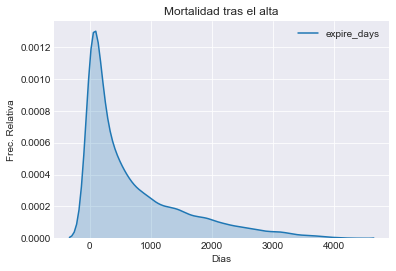
\includegraphics[scale= 0.68]{C:/mimic-iii-project/plots/Labels/expire_days.png}
\caption{Distribución de probabilidad de la mortalidad tras el alta}
\end{figure}

\begin{longtable}[]{@{}ll@{}}
\toprule
Descriptor estadístico & Valor\tabularnewline
\midrule
\endhead
Recuento & 16548 registros\tabularnewline
Media aritmética ($\mu$) & 708 días\tabularnewline
Desviación estándar ($\sigma$) & 820 días\tabularnewline
Valor mínimo & 0.5 días\tabularnewline
Percentil 25\% & 88 días\tabularnewline
Percentil 50\% & 374 días\tabularnewline
Percentil 75\% & 1067 días\tabularnewline
Valor máximo & 4327 días\tabularnewline
\bottomrule
\end{longtable}

Actualmente, los estudios llevados a cabo en este campo no han sido capaces de obtener resultados clínicamente significativos mediante modelos de regresión, es decir, no ha sido posible hasta el momento obtener el valor numérico del tiempo de supervivencia de los pacientes tras su alta. Esto se debe a la gran complejidad de los datos y sus relaciones subyacentes. El trabajo en este ámbito hasta el momento se ha centrado en tareas de clasificación binaria o multiclase. De esta forma, tras explorar la información y sus estadísticas, se decide clasificar los pacientes en los siguientes tres grupos de supervivencia.

\begin{longtable}[]{@{}lll@{}}
\toprule
Mortalidad & Cantidad & Porcentaje\tabularnewline
\midrule
\endhead
12+ meses & 8391 & 37 \%\tabularnewline
1-12 meses & 6095 & 27 \%\tabularnewline
\textless{} 1 mes & 8100 & 36 \%\tabularnewline
\bottomrule
\end{longtable}

La selección se ha realizado de forma expresa para evitar clases descompensadas que dificulten la predicción posterior. Así mismo, se trata de una agrupación de utilidad en la práctica clínica.
\newpage
 Por ejemplo, en caso de llevarse a producción el modelo y predecir que un paciente tiene altas probabilidades de morir en menos de un mes, el personal médico debería considerar la situación de este y su alta. Para ello, empleamos la siguiente consulta, la cual aplica directamente la clasificación en grupos mediante una sentencia CASE en SQL.

\begin{verbatim}
SELECT hadm_id,
	CASE
		WHEN
    		EXTRACT(epoch FROM (dod-dischtime))/(3600*24*30) > 12 
    	THEN '12+ months'
    	WHEN 
    		EXTRACT(epoch FROM (dod-dischtime))/(3600*24*30) < 12 AND
     		EXTRACT(epoch FROM (dod-dischtime))/(3600*24*30) >= 1

    	THEN '1-12 months'
    									
   		WHEN
    		EXTRACT(epoch FROM (dod-dischtime))/(3600*24*30) < 1 AND
    		EXTRACT(epoch FROM (dod-dischtime))/(3600*24*30) > -0.5
    	THEN '0-1 months'	
    									
    END
AS mortality
FROM admissions a
INNER JOIN patients p
ON a.subject_id = p.subject_id
\end{verbatim}
\newpage

\section{Variables predictorias}

A continuación, se recopilan una serie de variables determinantes a la hora de predecir el tiempo de
supervivencia tras el alta de la admisión hospitalaria. Las variables recopiladas se extraen a partir de consultas a la base de
datos y en algunos casos al preprocesamiento de estas. La distribución en clases atiende únicamente a criterios organizativos. 

\subsection{Información demográfica}

Se recopilan cinco variables de índole demográfica: Edad, sexo, estado
civil, religión y etnicidad. Estas variables se extraen directamente de
la tabla ADMISSIONS, excepto la edad, que se calcula a partir de la
diferencia de tiempo entre la fecha de nacimiento, almacenada en la
tabla PATIENTS, y la fecha de admisión hospitalaria, procedente de la
tabla ADMISSIONS.

\subsubsection{Edad}

La edad de los pacientes mayores a 91 años se encuentra desplazada en el
tiempo con la finalidad de proteger su identidad y dificultar su
identificación, en cumplimiento con la ley estadounidense de privacidad,
la HIPPA. De esta manera, encontramos con pacientes ancianos con edades
superiores a 300 años. Mediante una función de preprocesado substituimos
la edad de estos pacientes por 91 años. Posteriormente descartaremos
estos registros del conjunto de datos que servirá para entrenar la red
neuronal, por considerarlos poco fiables y propensos a inducir errores.
Así mismo, se descartarán igualmente los neonatos, por presentar un
comportamiento médico muy distinto al de la población adulta.
\begin{verbatim}
SELECT hadm_id, 
EXTRACT(epoch FROM (admittime dob))/(3600*24*365)
AS age
FROM admissions a
INNER JOIN patients p
ON a.subject_id = p.subject_id
\end{verbatim}

Se distribuye estadísticamente de la siguiente manera

\begin{figure}[h]
\centering
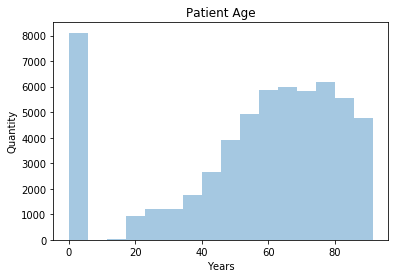
\includegraphics[scale = 0.70]{C:/mimic-iii-project/plots/Demographic_data/age_histogram.png}
\caption{Histograma de la distribución de la edad de los pacientes}
\end{figure}
\newpage
\begin{longtable}[]{@{}cc@{}}
\toprule
Descriptor estadístico & Valor (años)\tabularnewline
\midrule
\endhead
Recuento & 58976\tabularnewline
Media aritmética ($\mu$) & 55.2\tabularnewline
Desviación estándar ($\sigma$) & 27.3\tabularnewline
Valor mínimo & 0\tabularnewline
Percentil 25\% & 43.5\tabularnewline
Percentil 50\% & 61.8\tabularnewline
Percentil 75\% & 75.9\tabularnewline
Valor máximo & 91.4\tabularnewline
\bottomrule
\end{longtable}

\subsubsection{Sexo}

Extraemos esta variable para cada admisión hospitalaria directamente de la base de datos, sin ningún tipo de preprocesado, mediante la siguiente consulta simple. 
\begin{verbatim}
SELECT hadm_id, gender
FROM admissions a
INNER JOIN patients p
ON a.subject_id = p.subject_id
\end{verbatim}

Se distribuye de la siguiente manera

\begin{longtable}[]{@{}lll@{}}
\toprule
 & Recuento & Proporción\tabularnewline
\midrule
\endhead
Hombres & 39250 & 55.8\% \tabularnewline
Mujeres & 26026 & 44.2\% \tabularnewline
\bottomrule
\end{longtable}

\subsubsection{Estado Civil}

Lo obtenemos mediante la siguiente consulta, de forma análoga al sexo del paciente.

\begin{verbatim}
SELECT hadm_id, marital_status
FROM admissions a
INNER JOIN patients p
ON a.subject_id = p.subject_id
\end{verbatim}
Observamos clases claramente descompensadas y poco significativas que es conveniente tratar. 

\begin{longtable}[]{@{}ll@{}}
\toprule
Estado civil & Cantidad\tabularnewline
\midrule
\endhead
DIVORCED & 3213\tabularnewline
LIFE PARTNER & 15\tabularnewline
MARRIED & 24239\tabularnewline
SEPARATED & 571\tabularnewline
SINGLE & 13254\tabularnewline
UNKNOWN (DEFAULT) & 345\tabularnewline
WIDOWED & 7211\tabularnewline
\bottomrule
\end{longtable}

Para el preprocesado de esta variable, unificamos aquellos grupos de
características similares. En concreto, se juntan los grupos DIVORCED y
SEPARATED en uno solo, y se incluye LIFE PARTNER dentro de MARRIED. Para
realizar este agrupamiento se tienen en cuenta los hábitos de vida y factores socialdemográficos que pueden caracterizar a cada grupo. Tras realizar esta
agrupación, llegamos a las siguientes clases:
\newpage
\begin{longtable}[]{@{}ll@{}}
\toprule
Estado civil & Cantidad\tabularnewline
\midrule
\endhead
DIVORCED/SEPARATED & 3784\tabularnewline
MARRIED & 24254\tabularnewline
SINGLE & 13254\tabularnewline
UNKNOWN & 10473\tabularnewline
WIDOWED & 7211\tabularnewline
\bottomrule
\end{longtable}

\subsubsection{Religión}
Realizamos un procedimiento análogo al llevado a cabo en la variable
MARITAL\_STATUS, teniendo en cuenta las mismas consideraciones en el
momento de unificar grupos. Extraemos la variable de la base de datos
con la siguiente consulta
\begin{verbatim}
SELECT hadm_id, religion 
FROM admissions a
INNER JOIN patients p
ON a.subject_id = p.subject_id
\end{verbatim}
De la misma manera que con el estado civil, obtenemos grupos descompensados y poco significativos. En concreto, obtenemos 20 grupos, 14 de los cuales cuentan con menos de mil registros, de un total de $\sim$ 59.000. Tras agruparlos según características culturales similares, llegamos a los siguientes grupos:
\begin{longtable}[]{@{}lc@{}}
\toprule
Religion & Valores\tabularnewline
\midrule
\endhead
BUDDHIST/HINDU & 380\tabularnewline
CHRISTIAN & 29323\tabularnewline
JEWISH/HEBREW & 5330\tabularnewline
MUSLIM & 225\tabularnewline
NONE & 23176\tabularnewline
ORTHODOX & 542\tabularnewline
\bottomrule
\end{longtable}


\subsubsection{Etnicidad}

Realizando el mismo proceso que para las variables anteriores, extraemos
y unificamos la etnicidad del paciente para cada admisión hospitalaria.
\begin{verbatim}
SELECT hadm_id, ethnicity
FROM admissions a
INNER JOIN patients p
ON a.subject_id = p.subject_id
\end{verbatim}

Se recopilan 41 orígenes étnicos distintos, algunos muy similares entre si. Por ejemplo, se hace distinción de hispanos según el país, dando lugar a numerosas categorías con menos de diez entradas. Sucede lo mismo con pacientes de origen asiático y caucásico. También hay presentes registros de pacientes con origen nativo de Norteamérica (72 registros) o nativo del caribe (9 registros). Estos registros poco significativos se agrupan bajo la categoría OTHER. El resultado de preprocesar la variable es el siguiente:

\begin{longtable}[]{@{}ll@{}}
\toprule
Etnicidad & Cantidad\tabularnewline
\midrule
\endhead
ASIAN & 2007\tabularnewline
BLACK & 5785\tabularnewline
HISPANIC & 2136\tabularnewline
NONE & 5896\tabularnewline
OTHER & 1766\tabularnewline
WHITE & 41386\tabularnewline
\bottomrule
\end{longtable}

\subsection{Pruebas de laboratorio}

Se extraen diez pruebas de laboratorio comunes, realizadas
rutinariamente tras el ingreso de un paciente, para emplearlas como
variables predictorias. Para cada una de ellas, obtenemos su valor medio y su desviación
estándar, dando lugar a un total de veinte variables. Cada uno de los resultados de las pruebas se almacena en la tabla
LABEVENTS mediante un identificador, ITEMID.

La relación de ITEMIDs para las pruebas de laboratorio es la siguiente:

\begin{longtable}[]{@{}ll@{}}
\toprule
Prueba de laboratorio & ITEMID\tabularnewline
\midrule
\endhead
Nitrógeno ureico en sangre & 51066\tabularnewline
Recuento de plaquetas & 51265\tabularnewline
Hematocrito & 51221\tabularnewline
Potasio en sangre & 50971\tabularnewline
Sodio en sangre & 50983\tabularnewline
Creatinina en sangre & 50912\tabularnewline
Bicarbonato en sangre & 50882\tabularnewline
Recuento de leucocitos & 51301\tabularnewline
Glucosa en sangre & 50809, 50931\tabularnewline
Albúmina en sangre & 50862\tabularnewline
\bottomrule
\end{longtable}

Para obtener el promedio y la desviación estándar de cada una de estas
variables, por ejemplo para el sodio en sangre, realizamos la siguiente
consulta:

\begin{verbatim}
SELECT hadm_id,
avg(valuenum) AS AVG_SODIUM,
stddev(valuenum) AS STD_SODIUM,
FROM labevents
WHERE itemid = 50983
GROUP BY hadm_id
\end{verbatim}
Esta función se ejecuta en bucle para todas las pruebas de laboratorio.
En cuanto al preprocesado, descartamos aquellos valores por debajo del
percentil 1\% y por encima del percentil 99\%, al considerarlos errores
aberrantes o fallos de medición, además de ser poco significativos. Se
realiza mediante una función creada para ello.

Tras extraer las variables y tratarlas, obtenemos el siguiente
resultado:



\begin{longtable}[]{@{}cccccccccc@{}}
\toprule
Prueba  & Medidas (x10\textsuperscript{3}) & $\mu$ &
$\sigma$ & mín. &  P\textsubscript{25\%} & 
 P\textsubscript{50\%} &   P\textsubscript{75\%} & máx. & Unidad \tabularnewline
\midrule
\endhead
Nitrógeno ureico & 49.9 & 24.5 & 16.1 & 5.6 & 13.4 & 19.2 &
30.3 & 93 & mg/24hr\tabularnewline
Recuento de plaquetas & 55.8 & 241.1 & 97.9 & 44.9 & 172.3 & 229 & 297.1
& 595.6 & K/uL\tabularnewline
Hematocrito & 55.9 & 33.9 & 6.9 & 23.8 & 29.1 & 31.9 & 36.7 & 58.9 &
\%\tabularnewline
Potasio en sangre & 51.8 & 4.2 & 0.4 & 3.3 & 3.9 & 4.1 & 4.4 & 5.8 &
mEq/L\tabularnewline
Sodio en sangre & 51.8 & 138.7 & 3.1 & 128.7 & 136.9 & 138.9 & 140.8 &
147.8 & mEq/L\tabularnewline
Creatinina en sangre & 49.9 & 1.3 & 1.1 & 0.35 & 0.72 & 0.93 & 1.34 &
7.9 & mg/dL\tabularnewline
Bicarbonato en sangre & 51.8 & 138.7 & 3.1 & 128.7 & 136.9 & 138.9 &
140.8 & 147.8 & mEq/L\tabularnewline
Recuento de leucocitos & 55.8 & 241 & 97.9 & 44.9 & 172.3 & 229 & 297.1
& 595.6 & K/uL\tabularnewline
Glucosa en sangre & 49.6 & 131.7 & 32.9 & 78.2 & 110 & 124.2 & 124.3 &
144.3 & mg/dL\tabularnewline
Albúmina en sangre & 30.5 & 3.2 & 0.6 & 1.7 & 2.7 & 3.2 & 3.7 & 4.7 &
g/dL\tabularnewline
\bottomrule
\end{longtable}
\newpage
\subsection{Señales fisiológicas}

De la misma forma que obtenemos los resultado de las pruebas de
laboratorio, extraemos de la base de datos el promedio y la desviación
estándar de seis señales fisiológicas para emplearlas como variables
predictorias.

Las medidas han sido tomadas con dos sistemas de monitorización
distintos, Philips CareVue y Metavision. Así mismo, la base de datos
distingue entre medidas tomadas automáticamente y medidas tomadas
expresamente por el personal médico, entre otros factores. Es por ello
que una misma medida presenta múltiples identificadores.

\begin{longtable}[]{@{}ll@{}}
\toprule
Señal fisiológica & ITEMID\tabularnewline
\midrule
\endhead
Frecuencia cardíaca & 220045, 211\tabularnewline
Frecuencia respiratoria & 8113, 3603, 220210, 618\tabularnewline
Presión sistólica & 51,442,455,6701,220179,220050\tabularnewline
Presión díastólica & 8368,8440,8441,8555,220180,220051\tabularnewline
Temperatura & 223761,678\tabularnewline
Saturación de oxígeno & 646, 220277\tabularnewline
\bottomrule
\end{longtable}

Las señales fisiológicas se registran en la tabla CHARTEVENTS. Empleamos
la siguiente consulta, muy similar a la empleada para obtener los
resultados de las pruebas de laboratorio. Por ejemplo, para extraer los valores
deseados en el caso de la saturación de oxígeno utilizaríamos la siguiente consulta.

\begin{verbatim}
SELECT hadm_id, avg(valuenum) AS AVG_SPO2, stddev(valuenum) AS STD_SPO2,
FROM chartevents WHERE itemid IN (646, 220277) GROUP BY hadm_id
\end{verbatim}

Aplicamos el mismo procesamiento usado anteriormente, es decir, descartamos aquellos valores por debajo del percentil 1\% y aquellos por encima del 99\%. La estadísticas descriptivas del promedio de estas variables son las siguientes:
\begin{longtable}[]{@{}llllllllll@{}}
\toprule
Prueba  & Medidas (x10\textsuperscript{3}) & $\mu$ &
$\sigma$ & mín. &  P\textsubscript{25\%} & 
 P\textsubscript{50\%} &   P\textsubscript{75\%} & máx. & Unidad \tabularnewline
\midrule
\endhead
Frecuencia cardíaca & 55.6 & 92.2 & 22.9 & 55.5 & 78.9 & 86.8 & 99.8 &
162 & BPM\tabularnewline
Frecuencia respiratoria & 55.6 & 22.7 & 10.1 & 12.4 & 16.9 & 19.4 & 23 &
60 & BPM\tabularnewline
Presión sistólica & 48 & 120.5 & 15.2 & 86.8 & 109.2 & 118.8 & 130.6 &
163.8 & mmHg\tabularnewline
Presión díastólica & 48 & 61 & 9.7 & 39.2 & 54 & 60.1 & 67.1 & 91.8 &
mmHg\tabularnewline
Temperatura & 47.2 & 98.2 & 0.9 & 94.7 & 97.7 & 98.2 & 98.8 & 100.6 &
ºF\tabularnewline
Saturación de oxígeno & 48 & 96.9 & 1.64 & 89.3 & 96.1 & 97.2 & 98.8 &
99.8 & \%\tabularnewline
\bottomrule
\end{longtable}

\begin{figure}[H]
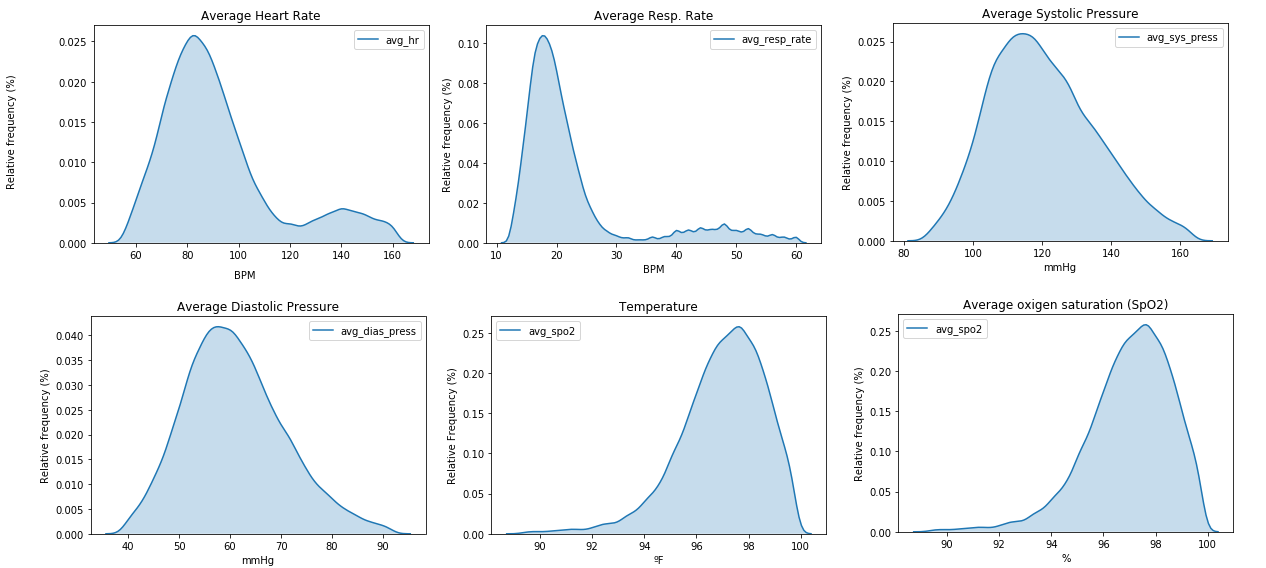
\includegraphics[scale=0.50]{C:/mimic-iii-project/plots/Physio_data/subplot.png}
\caption{Distribución de probabilidad de las señales fisiológicas extraídas}
\end{figure}

\subsection{Información hospitalaria}

Se extraen once variables relacionadas con cada estancia hospitalaria.

\begin{longtable}[]{@{}ll@{}}
\toprule
Variables hospitalarias & Tipo\tabularnewline
\midrule
\endhead
Servicio médico & Categórica (20 valores)\tabularnewline
Grupo de diagnóstico ICD9 & Categórica\tabularnewline
Realización de cirugía & Binaria\tabularnewline
Duración de estancia en UCI & Numérica continua\tabularnewline
Duración de estancia total & Numérica continua\tabularnewline
Indicador de severidad OASIS & Numérica entera\tabularnewline
Indicador de severidad SAPS & Numérica entera\tabularnewline
Indicador de severidad SOFA & Numérica entera\tabularnewline
Tiempo en ventilación mecánica & Numérica continua\tabularnewline
Fallecimiento en hospital & Binaria\tabularnewline
Cantidad de procedimientos realizados & Numérica entera\tabularnewline
\bottomrule
\end{longtable}
\paragraph{Servicio médico}
Se trata de una variable categórica que indica el servicio médico más
relevante por el cual es atendido el paciente en la estancia
hospitalaria. Debido a que en numerosas ocasiones un paciente permanece
en más de un servicio durante su estancia, es necesario una función de
preprocesado que extraiga el servicio de mayor importancia en función de
un criterio.

En concreto, se ha diseñado una función que utiliza la siguiente
prioridad para extraer un único servicio para cada estancia
hospitalaria.

\begin{itemize}
\item
  Servicios de cirugía especializada 
\item
  Servicio de cirugía general
\item
  Servicio especializado
\item
  Servicio de medicina general
\end{itemize}

De esta forma, un paciente admitido en el servicio de medicina general y
posteriormente trasladado al servicio de cirugía cardíaca, constará como
un paciente tratado bajo el servicio de cirugía cardíaca únicamente, por
ejemplo. Esto permite reducir la dimensionalidad de la variable y obtener la
información de mayor relevancia. Tras aplicar este preprocesado, se
obtienen las siguientes categorías y recuentos.

\begin{longtable}[]{@{}lll@{}}
\toprule
Servicio médico & Significado & Cantidad\tabularnewline
\midrule
\endhead
MED & Medicina general & 17260\tabularnewline
NB & Neonatos & 7806\tabularnewline
CSURG & Cirugía cardíaca & 7697\tabularnewline
CMED & Cardiología & 5860\tabularnewline
SURG & Cirugía general & 5034\tabularnewline
NSURG & Cirugía neurológica & 4024\tabularnewline
TRAUM & Traumatología & 2699\tabularnewline
NMED & Neurología & 2324\tabularnewline
OMED & Obstetricia & 1475\tabularnewline
VSURG & Cirugía vascular no cardíaca & 1371\tabularnewline
TSURG & Cirugía torácica & 1281\tabularnewline
ORTHO & Ortopedia & 739\tabularnewline
GU & Urología & 334\tabularnewline
PSURG & Cirugía plástica & 269\tabularnewline
GYN & Ginecología & 206\tabularnewline
\bottomrule
\end{longtable}
\newpage
\paragraph{Grupo de diagnóstico ICD-9}


ICD-9 es el acrónimo de "International Statistical Classification of
Diseases and Related Health Problems 9th Revision", publicado por la
Organización Mundial de la Salud en 1977.

Se emplean para clasificar y codificar las patologías, lesiones,
síntomas, circunstancias sociales y causas externas de enfermedades, con
el fin de recopilar información sanitaria útil relacionada con
defunciones, enfermedades y traumatismos. Estos códigos se dividen en capítulos, secciones, categorías,
subcategorías y subclasificaciones, por ejemplo:

\newlist{myEnumerate}{enumerate}{5}
\setlist[myEnumerate,1]{label=(\arabic*)}
\setlist[myEnumerate,2]{label=(\Roman*)}
\setlist[myEnumerate,3]{label=(\Alph*)}
\setlist[myEnumerate,4]{label=(\roman*)}
\setlist[myEnumerate,5]{label=(\alph*)}


\begin{myEnumerate}
\item   Códigos 390 -- 459: Enfermededades del sistema circulatorio
    \begin{myEnumerate}
    \item Enfermedades cerebrovasculares (430-438)
        \begin{myEnumerate}
        \item Oclusión de arterias cerebrales (434)
            \begin{myEnumerate}
            \item Embolia cerebral (434.1)
                \begin{myEnumerate}
                \item Embolia cerebral con infarto cerebral (434.1.1)
                \end{myEnumerate}
            \end{myEnumerate}
         \end{myEnumerate}
      \end{myEnumerate}
\end{myEnumerate}

La versión más actual es la ICD-10, que se desarrolló en 1992, aunque en
la base de datos MIMIC III v1.4 se recoge la versión anterior, la ICD-9.
Actualmente, se está realizando la transición generalizada a nivel
mundial del estándar ICD -- 9 a ICD -- 10. Debido a la gran variedad de códigos y al desbalance de clases de cada
código específico, se emplea únicamente el código primario ICD -- 9, tal
y como se recogen en el siguiente listado:

\begin{itemize}
\item
  Codigos 001 -- 139: Enfermedades infecciosas y parasitarias
\item
  Códigos 140 -- 239: Neoplasias
\item
  Códigos 240 - 279 : Enfermedades endocrinas, de la nutrición y
  metabólicas y trastornos de la inmunidad
\item
  Códigos 280 -- 289: Enfermedades de la sangre y de los órganos
  hematopoyéticos
\item
  Códigos 290 -- 319: Trastornos mentales
\item
  Códigos 320 -- 389: Enfermedades del sistema nervioso y de los órganos
  de los sentidos
\item
  Códigos 390 -- 459: Enfermedades del sistema circulatorio
\item
  Códigos 460 -- 519: Enfermedades del aparato respiratorio
\item
  Códigos 520 -- 579: Enfermedades del aparato digestivo
\item
  Códigos 580 -- 629: Enfermedades del aparato genitourinario
\item
  Códigos 630 -- 679: Complicaciones del embarazo, parto y puerperio
\item
  Códigos 680 -- 709: Enfermedades de la piel y del tejido subcutáneo
\item
  Códigos 710 -- 739: Enfermedades del sistema osteo-mioarticular y
  tejido conjuntivo
\item
  Códigos 740 -- 759: Anomalías congénitas
\item
  Códigos 760 -- 779: Ciertas enfermedades con origen en el periodo
  perinatal
\item
  Códigos 780 -- 799: Síntomas, signos y estados mal definidos
\item
  Códigos 800 -- 999: Lesiones y envenenamientos
\item
  Códigos E y V: Causas externas de lesiones y clasificación
  suplementaria. 
\end{itemize}

Mediante la siguiente consulta obtenemos el código ICD-9 de mayor
prioridad para cada admisión, indicado por seq\_num = 1 en la base de datos.

\begin{verbatim}
SELECT hadm_id, diagnoses_icd.icd9_code
FROM diagnoses_icd  
INNER JOIN d_icd_diagnoses 
ON diagnoses_icd.icd9_code = d_icd_diagnoses.icd9_code 
WHERE seq_num = 1
\end{verbatim}

Es necesaria una función de filtrado que convierta el código ICD-9
específico a su clasificación mayor en función de su número de código,
lo cual se realizará en la etapa de preprocesado.

\paragraph{Realización de cirugía}

Para detectar si se han realizado intervenciones quirúrgicas en un
paciente durante su estancia hospitalaria emplearemos los indicadores de
cirugía, (Surgery Flags), proporcionados por el HCUP, Healthcare Cost
and Utilization Project, una iniciativa financiada por el gobierno
estadounidense mediante la `Agency for Healthcare Research and Quality'
(AHRQ) dedicada a la gestión y análisis de datos médicos.

Esta entidad proporciona herramientas para identificar intervenciones y
eventos quirúrgicos mediante códigos ICD-9 de procedimiento o códigos CPT
(Current Procedural Terminology) , ambos presentes en la base de datos
MIMIC-III v.1.4.
Permite la clasificación de procedimientos en tres grupos:

\begin{itemize}
\item
  NARROW: Procedimientos quirúrgicos terapéuticos invasivos requiriendo
  incisión, extirpación, manipulación o suturado de tejido que penetra o
  atraviesa la piel, típicamente se realiza en quirófano y con anestesia
  local o general o sedación.
\item
  BROAD: Procedimientos quirúrgicos que no se pueden clasificar como
  aquellos incluidos en el indicador NARROW, pero se realizan bajo
  condiciones quirúrgicas. Este grupo incluye procedimientos quirúrgicos
  de diagnóstico, como procedimientos endoscópicos o percutáneos, o
  aquellos realizados a través de orificios naturales. Se trata de
  intervenciones menos invasivas.
\item
  NEITHER: Procedimientos no registrado como NARROW o BROAD, es decir,
  procedimientos no quirúrgicos. 
\end{itemize}

Esta clasificación se distribuye en forma de archivo CSV y mediante
Python se diseña una función para devolver la clasificación del
procedimiento.
Debido a que únicamente se clasifican un 4\% de registros como BROAD, se
decide incluir estos dentro de NARROW con el fin de evitar clases
desproporcionadas, dando lugar a una variable binaria con la siguiente
distribución.

\begin{longtable}[]{@{}ccc@{}}
\toprule
Indicador de cirugía & Recuento & Porcentaje\tabularnewline
\midrule
\endhead
Narrow & 29867 & 56\%\tabularnewline
No Surgery & 23043 & 44\%\tabularnewline
\bottomrule
\end{longtable}

\paragraph{Duración de estancia en UCI}
De la base de datos es posible extraer directamente la duración de
estancia en UCI en días para cada paciente en una misma admisión
hospitalaria. Esta información se haya en la tabla ICUSTAYS y la
obtenemos mediante la siguiente consulta.

\begin{verbatim}
SELECT hadm_id, 
sum(los) AS total_icu_time 
FROM icustays
GROUP BY hadm_id
\end{verbatim}

Es necesario emplear la función agregada de suma en la consulta debido a
que en ciertas ocasiones un paciente ingresa en la UCI, es transferido a
otra sección y posteriormente regresa a la UCI, con lo cual se registran
distintas duraciones para una misma estancia. De esta forma, obtenemos
una variable continua, a la cual no aplicamos preprocesado.


\begin{figure}[H]
\centering
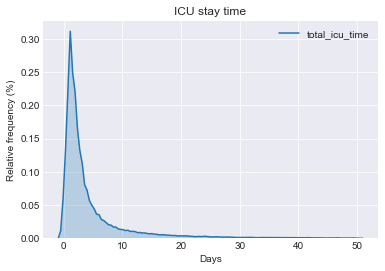
\includegraphics[scale = 0.65]{C:/mimic-iii-project/plots/ICU_data/icu_time.png}
\caption{Distribución de probabilidad de la estancia en UCI}
\end{figure}


\paragraph{Duración de estancia hospitalaria}

Obtenemos la duración de estancia hospitalaria, incluyendo la duración
en UCI, como la diferencia entre el tiempo de admisión y de alta. Para
ello empleamos la función EXTRACT y epoch, propias de PostgreSQL.

\begin{verbatim}
SELECT hadm_id, 
EXTRACT(epoch FROM(dischtime - admittime))/(3600*24) AS total_los_days
FROM admissions
\end{verbatim}
Esta variable se mide también en días y no requiere preprocesado. Se distribuye de la siguiente manera.

\begin{figure}[H]
\centering
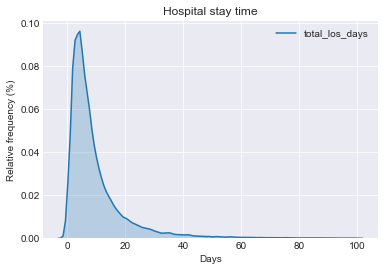
\includegraphics[scale = 0.65]{C:/mimic-iii-project/plots/ICU_data/los_time.png}
\caption{Distribución de probabilidad de la estancia hospitalaria completa}
\end{figure}

\paragraph{Recuento de admisiones}

Para cada admisión, indica la cantidad de estancias hospitalarias que ha
realizado el mismo paciente, contando también la misma. Esto permite identificar aquellas admisiones correspondientes a
pacientes readmitidos en diversas ocasiones, lo cual puede ser indicador
de sujetos con enfermedades crónicas, que requieren regularmente
atención médica. Obtenemos esta variable mediante funciones de preprocesado sobre la
tabla ADMISSIONS.

\paragraph{Recuento de procedimientos}
Indica la cantidad de procedimientos, tanto quirúrgicos como no
quirúrgicos, realizados a un paciente en una misma estancia
hospitalaria. Se trata de una variable numérica discreta que obtenemos
mediante la siguiente consulta.

\begin{verbatim}
SELECT hadm_id, count(*) AS procedure_count
FROM procedures_icd
GROUP BY hadm_id
\end{verbatim}
Esta variable no requiere preprocesado.

\paragraph{Tiempo en ventilación mecánica}

Empleando de nuevo una vista materializada disponible en el repositorio
de código de MIMIC-III, obtenemos el tiempo que pasa cada paciente en
ventilación mecánica durante su estancia hospitalaria. Utilizamos la
siguiente consulta sobre la vista VENTDURATIONS.

\begin{verbatim}
SELECT hadm_id, SUM(duration_hours) AS total_mech_vent_time
FROM ventdurations v
INNER JOIN icustays i
ON v.icustay_id = i.icustay_id
GROUP BY hadm_id
\end{verbatim}
En ocasiones, un paciente pasa un tiempo conectado al ventilador
mecánico, es desconectado, y conectado de nuevo posteriormente. Es por
ello que la vista materializada registra en ocasiones diversas entradas
para una misma estancia en UCI, con lo cual es conveniente calcular la
suma de duraciones para una estancia.

\subsubsection{Indicadores de severidad}
Distintos indicadores de severidad han sido desarrollados con el
objetivo y predecir la mortalidad hospitalaria a partir de la
información de los pacientes, en particular de las medidas tomadas
durante las primeras 24h horas de su ingreso. Sin embargo, presentan
ciertas limitaciones, por ejemplo al depender de medidas subjetivas
tomadas por el personal médico o al emplear relaciones lineales que no
se adaptan a la realidad.

Utilizaremos como variables predictoras los indicadores SOFA, SAPS y
OASIS, los cuales obtendremos mediante la siguiente consulta:

\begin{verbatim}
SELECT o.hadm_id, 
AVG(o.oasis) AS oasis_avg, 
AVG(so.sofa) AS sofa_avg, 
AVG(sa.saps) as saps_avg
FROM oasis o
INNER JOIN sofa so
ON o.hadm_id = so.hadm_id
INNER JOIN saps sa
ON sa.hadm_id = so.hadm_id
GROUP BY o.hadm_id
\end{verbatim}

Para obtener estos indicadores, utilizamos scripts del repositorio de
código oficial de MIMIC-III.
{[}https://github.com/MIT-LCP/mimic-code/tree/master/concepts/severityscores{]}.
De esta manera, creamos vistas materializadas que contienen los
indicadores de severidad precalculados para cada admisión hospitalaria.

\paragraph{SOFA}

``Sequential Organ Failure Assessment score''. Creado en 1994 por la
European Society of Intensive Medicine (ESICM), este indicador fue
desarrollado para evaluar la severidad de la enfermedad del paciente,
basada en el grado de fallo orgánico de seis órganos. En concreto, se
toman las siguientes medidas.

\begin{itemize}
\item
  Sistema respiratorio:
\item
  \begin{itemize}
  \item
    PaO2
  \item
    Presencia de ventilación mecánica
  \end{itemize}
\item
  Sistema nervioso:
\item
  \begin{itemize}
  \item
    Glasgow Coma Scale. 
  \end{itemize}
\item
  Sistema cardiovascular:
\item
  \begin{itemize}
  \item
    Presión arterial media
  \item
    Nivel de dopamina
  \item
    Nivel de Epinefrina
  \item
    Nivel de norepinefrina
  \end{itemize}
\item
  Hígado:
\item
  \begin{itemize}
  \item
    Nivel de bilirrubina
  \end{itemize}
\item
  Coagulación:
\item
  \begin{itemize}
  \item
    Nivel de plaquetas
  \end{itemize}
\item
  Renal:
\item
  \begin{itemize}
  \item
    Nivel de creatinina
  \item
    Volumen de orina
  \end{itemize}
\end{itemize}

Los resultados de estas pruebas otorgan puntuaciones entre 0 y 4, que
posteriormente se suman para obtener la puntuación SOFA total. Permite
obtener una idea aproximada de la mortalidad del paciente, de manera
sencilla y directa de calcular a partir de solamente once variables
básicas.
\paragraph{SAPS}

``Simplified Acute Physiology Score". Creado en 1993 por Le Gall y
Lemenshow Saulnier, se emplea para medir la severidad de la enfermedad
de los paciente admitidos en unidad de cuidados intensivos de edad mayor
a 15 años. Se completa 24h tras el ingreso y otorga una puntuación de
entre 0 y 163, además de la mortalidad predicha en porcentaje. Se
calcula a partir de 12 medidas fisiológicas básicas, la edad del
paciente y el tipo de admisión.

El resultado de SAPS es mejor empleado para contrastar la gravedad de
grupos de pacientes con patologías distintas, más que a nivel
individual, debido a que sus resultados pueden ser poco precisos a nivel
de paciente.

\paragraph{OASIS}

``Oxford Acute Severity of Illness Score", se trata de un indicador
de severidad diseñado en 2013 por Johnson AE1, Kramer AA, Clifford GD,
de la Universidad de Oxford. Se caracteriza por emplear técnicas de
aprendizaje automático, en concreto optimización por enjambre de
partículas, y por no requerir un gran trabajo de recolección de
información, ya que requiere únicamente diez características, excluyendo
medidas de laboratorio, o información sobre diagnósticos y
comorbilidades.

\paragraph{Escala de coma de Glasgow}

Se trata de una escala neurológica diseñada para medir fácilmente y de
forma objetiva el estado de consciencia de una persona. Un paciente es
puntuado según unos criterios en diversos aspectos, y la suma de
puntuaciones otorga una puntuación entre 3, indicando profunda
inconsciencia, y 14, indicando un estado de alerta normal.

Se emplea también como variable para calcular los indicadores de
severidad OASIS, SAPS y SOFA. Se obtiene siguiendo los criterios
siguientes:

\begin{figure}[H]
\centering
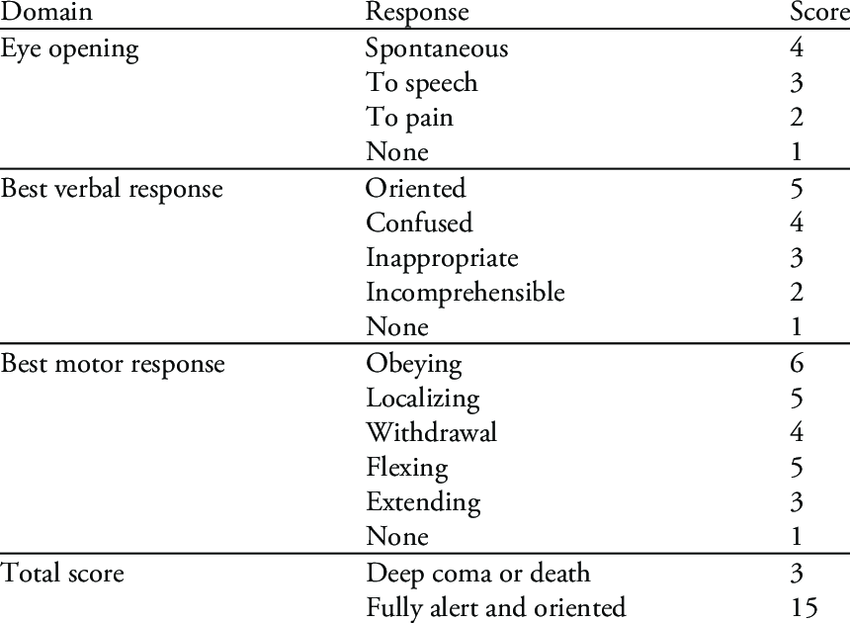
\includegraphics[scale = 0.30]{C:/mimic-iii-project/plots/glasgow_coma_scale.png}
\caption{Parámetros para calcular el valor de coma de Glasgow}
\end{figure}

\paragraph{Tiempo en ventilación mecánica}
Empleando de nuevo una vista materializada disponible en el repositorio
de código de MIMIC-III, obtenemos el tiempo que pasa cada paciente en
ventilación mecánica durante su estancia hospitalaria. Utilizamos la
siguiente consulta sobre la vista VENTDURATIONS.

\begin{verbatim}
SELECT hadm_id, SUM(duration_hours) AS total_mech_vent_time
FROM ventdurations v
INNER JOIN icustays i
ON v.icustay_id = i.icustay_id
GROUP BY hadm_id
\end{verbatim}

En ocasiones, un paciente pasa un tiempo conectado al ventilador
mecánico, es desconectado, y conectado de nuevo posteriormente. Es por
ello que la vista materializada registra en ocasiones diversas entradas
para una misma estancia en UCI, con lo cual es conveniente calcular la
suma de duraciones para una estancia.

\chapter{Modelo predictivo}

Las redes neuronales utilizan formas de procesamiento análogas a las del cerebro humano como base para desarrollar algoritmos capaces de hallar relaciones complejas no lineales entre variables de entrada y salida.
Esto permite la creación de modelos predictivos capaces de aprender de la información proporcionada y generalizar los resultados para realizar nuevas predicciones. 
A diferencia de otras formas de crear modelos predictivos, las redes neuronales artificiales no imponen ningún tipo de restricción sobre las variables de entrada, como su distribución.
También han demostrado un rendimiento superior en gran variedad de tareas respecto a métodos clásicos de aprendizaje automático.

Otra gran ventaja es su facilidad para escalar su capacidad predictiva en función de la cantidad de información que recibe, permitiendo mayores precisión simplemente añadiendo más datos de entrada. Así mismo, eliminan la necesidad de tratar extensamente las variables de entrada del modelo, no siendo necesario realizar un gran análisis exploratorio para determinar que variables són más relevantes y cuales se deben excluir, ni crear variables nuevas a partir de combinaciones de las ya existentes.

\begin{figure}[h]
\centering
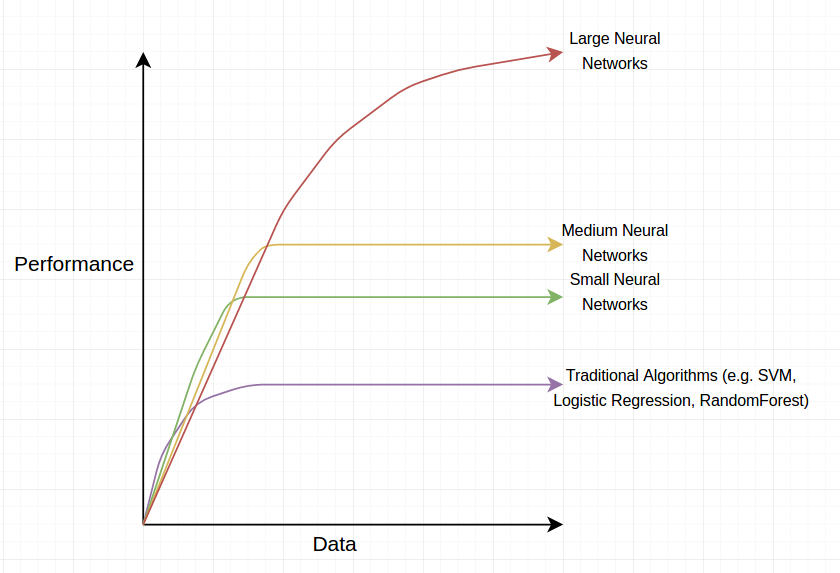
\includegraphics[scale = 0.40]{C:/mimic-iii-project/plots/deep_learning.png}
\caption{Comparativa de rendimiento de distintos métodos para crear modelos predictivos}
\end{figure}

Sin embargo, las redes neuronales son computacionalmente costosas y actuan como modelo caja negra, siendo difícil extraer y entender las relaciones que ha creado el modelo.  Dado que la información presente en la base de datos MIMIC-III v1.4 presenta relaciones complejas y disponemos de un volumen de datos adecuados, se decide emplear una red neuronal artificial para crear un modelo predictivo para la mortalidad extrahospitalaria.
\newpage
\section{Tecnologías utilizadas}

Para tratar y preprocesar la información, además de para crear el modelo predictivo, se pretende emplear el lenguaje de programación Python, en su versión 3.6. Se ha decidido emplear este lenguaje por poseer experiencia anterior en su uso, además de existir una gran comunidad dedicada a su uso en análisis y minería de datos, junto con potentes librerías y amplio soporte. 
El diseño de la red neuronal se construye con la librería Keras. Se trata de una librería de código abierto escrita capaz de ejecutarse sobre Tensorflow y Theano, principales librerías en cuanto a aprendizaje automático y redes neuronales; ofreciendo una API de alto nivel, modular y extensible. Incluye numerosas implementaciones de objetos usados comunmente en la construcción de redes neuronales artificiales, tal como capas, funciones de activación y optimizadores. Keras fue inicialmente desarrollado por François Chollet, ingeniero de Google, como parte de la investigación para el proyecto ONEIROS (Open-ended Neuro-Electronic Intelligent Robot Operating System) en 2016.
La información de MIMIC III v1.4 se almacena en una base de datos de PostrgreSQL, recomendada por los desarrolladores de MIMIC-III. Se trata de una base de datos relacional orientada a objetos y libre, creada inicialmente en 1995. En el repositorio oficial del proyecto MIMIC se hayan los scripts necesarios para cargar los archivos CSV, que contienen los datos de la base de datos, sobre PostgreSQL, además de los pasos para la creación de índices que agilizan las consultas. 
El preprocesado y tratamiento numérico de los datos se realiza con distintas librerías, principalmente con Pandas y Numpy,  paquete básicos para el análisis de datos en Python que proporcionan estructuras de datos diseñadas para trabajar con datos relacionales de forma rápida, flexible y fácil de entender, y Scikit-Learn, librería con diversas herramientas de aprendizaje automático de la cual empleamos sus funciones de preprocesado.


\begin{figure}[h]
\centering

\includegraphics[scale = 0.30]{C:/mimic-iii-project/plots/pylogo.png}
\caption{Logotipo de Python}
\end{figure}
\section{Preparación de datos}
Para obtener un rendmiento óptimo de la red neuronal, los datos de entrada deben ser tratados. Principalmente, deben tratarse los datos faltantes, normalizar las variables numéricas para que se encuentren en rangos similares, y deconstruir las variables categóricas en variables binarias para cada una de sus clases. 

\subsection{Imputación de valores faltantes (MICE)}
Es común encontrar valores faltantes en la base de datos MIMIC III. Por ejemplo, es posible que aun paciente determinado no se le haya realizado alguna prueba de laboratorio, o no se le haya tomado cierta medida fisiológica por algún motivo. Es necesario que los datos de entrada de la red neuronal se encuentren completos con el fin de poder construir el modelo predictivo. 

Existen diversas maneras de enfocar esta problemática. Una posibilidad es eliminar todos los registros con algún valor faltante, aunque en este caso no es viable debido al gran número de variables, lo cual hace que más del 95\% de registros tengan por lo menos un valor faltante, reduciendo de esta forma el conjunto de datos a menos de 200 registros completos. Esta cantidad no permitiría entrenar correctamente la red neuronal. Por otra parte, también pueden sustituirse los valores faltantes por su promedio o su moda, aunque esto reduce la variabilidad del conjunto de datos y es posible cometer errores importantes. 

Finalmente, se decide imputar los valores faltantes mediante la técnica MICE (Multivariate Imputation by Chained Equations). Se trata de un proceso iterativo que construye un modelo de imputación para cada variable mediante una serie de modelos de regresión, a partir de los datos observados y sus relaciones existentes. Para ello, utilizamos la librería 'fancyimpute': [https://github.com/iskandr/fancyimpute].

Tras realizar la imputación, se calcula el error cuadrático medio de imputación para cada variable, al imputar 200 valores previamente conocidos. Eso permite validar que la imputación ha producido un resultado adecuado. 
\begin{longtable}[]{@{}lrrr@{}}
\toprule
Variable & \% Error & Número de imputaciones & \% Valores
imputados\tabularnewline
\midrule
\endhead
std\_blood\_urea\_nitrogen & 64 & 9432 & 15\tabularnewline
std\_platelet\_count & 57 & 8503 & 14\tabularnewline
std\_white\_blood\_cells & 51 & 8629 & 14\tabularnewline
avg\_blood\_urea\_nitrogen & 50 & 9036 & 15\tabularnewline
avg\_creatinine & 49 & 9039 & 15\tabularnewline
total\_icu\_time & 46 & 1312 & 2.2\tabularnewline
avg\_platelet\_count & 41 & 3185 & 5.2\tabularnewline
std\_sodium & 41 & 8426 & 14\tabularnewline
std\_blood\_glucose & 39 & 9541 & 16\tabularnewline
std\_temp & 37 & 13060 & 21\tabularnewline
std\_hematrocrit & 36 & 8085 & 13\tabularnewline
std\_bicarbonate & 34 & 8467 & 14\tabularnewline
std\_hr & 32 & 5364 & 8.8\tabularnewline
std\_spo2 & 32 & 11170 & 18\tabularnewline
avg\_white\_blood\_cells & 31 & 3158 & 5.2\tabularnewline
std\_potasssium & 30 & 8321 & 14\tabularnewline
std\_resp\_rate & 23 & 5482 & 9\tabularnewline
std\_sys\_press & 22 & 11104 & 18\tabularnewline
std\_días\_press & 21 & 11134 & 18\tabularnewline
oasis\_avg & 19 & 1302 & 2.1\tabularnewline
sofa\_avg & 17.2 & 1302 & 2.1\tabularnewline
saps\_avg & 17 & 1302 & 2.1\tabularnewline
avg\_albumin & 14 & 29669 & 49\tabularnewline
std\_creatinine & 13.9 & 9430 & 15\tabularnewline
avg\_resp\_rate & 12 & 3540 & 5.8\tabularnewline
avg\_blood\_glucose & 11 & 9376 & 15\tabularnewline
avg\_hr & 10 & 3551 & 5.8\tabularnewline
avg\_días\_press & 10 & 11075 & 18\tabularnewline
avg\_bicarbonate & 9.6 & 7190 & 12\tabularnewline
avg\_sys\_press & 8.9 & 11075 & 18\tabularnewline
avg\_hematrocrit & 8.6 & 3046 & 5\tabularnewline
avg\_potasssium & 5.8 & 7189 & 12\tabularnewline
avg\_sodium & 2 & 7222 & 12\tabularnewline
avg\_spo2 & 1.2 & 11114 & 18\tabularnewline
avg\_temp & 0.57 & 11876 & 19\tabularnewline

\bottomrule

\caption {Error de los valores imputados}
\end{longtable}

\subsection{Normalización de variables numéricas}

Debido a que el rango de valores de los datos varia ampliamente, ciertas funciones podrían no funcionar correctamente sin la normalización de estos. Por ejemplo, la mayoría de clasificadores calculan la distancia entre dos puntos mediante la distancia euclídea. Si una de las dos características tiene un rango notablemente más amplio que otras, la distancia será marcada por esta característica, con lo cual su peso en el algoritmo será mucho mayor de lo que debería. Por lo tanto, el rango de todas las características debe ser normalizada con el fin de que cada variable contribuya de forma equilibrada. De la misma forma, la normalización de las variables permite que el descenso de gradiente, paso indispensable en una red neuronal, llegue a converger a mayor velocidad. 

Debido a esto, se normalizan todas las variables numéricas para que se asemejen a una distribución normal, dónde la media es cero y la desviación típica es uno. Realizamos este proceso mediante el método 'scale' del módulo 'preprocessing' de la librería 'Scikit Learn'

\begin{figure}[h]
\centering
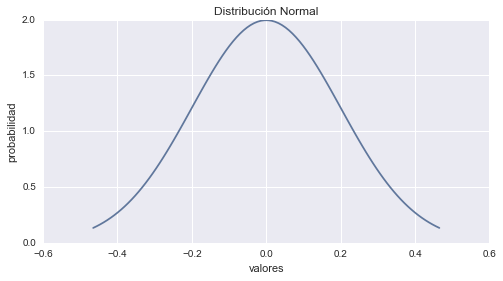
\includegraphics[scale = 0.5]{C:/mimic-iii-project/plots/normal_distribution.png}
\caption{Distribución de probabilidad normal}
\end{figure}
\newpage

\subsection{Codificación de variables categóricas}

Las variables categóricas deben ser codificadas para ser aceptadas por
la red neuronal. En concreto, deben dividirse en columnas con valores
binarios para cada una de las clases que toma la variable.

\begin{longtable}[]{@{}cc@{}}
\toprule
ID\_Paciente & Mortalidad\tabularnewline
\midrule
\endhead
456 & \textless{} 1 mes\tabularnewline
321 & 1 - 12 meses\tabularnewline
678 & 12+ meses\tabularnewline
543 & 1 -12 meses\tabularnewline
987 & \textless{} 1 mes\tabularnewline
\bottomrule
\end{longtable}

Por ejemplo, la tabla anterior se debe convertir al siguiente formato,
donde cada columna corresponde a un intervalo de mortalidad.

\begin{longtable}[]{@{}cccc@{}}
\toprule
ID\_Paciente & \textless{} 1 mes & 1 - 12 meses & 12+
meses\tabularnewline
\midrule
\endhead
456 & 1 & 0 & 0\tabularnewline
321 & 0 & 1 & 0\tabularnewline
678 & 0 & 0 & 1\tabularnewline
543 & 0 & 1 & 0\tabularnewline
987 & 1 & 0 & 0\tabularnewline
\bottomrule
\end{longtable}
Realizamos este proceso tanto para la variable a predecir, mortalidad extrahospitalaria, como para aquellas variables predictorias categóricas,
tales como la etnicidad del paciente, religión, o el grupo de código de
diagnósticos ICD9, entre otras.
Se lleva a cabo mediante el método get\_dummies de la librería de
cálculo numérico Pandas.

\subsection{División en conjunto de entrenamiento y
evaluación}

Es conveniente dividir el conjunto de datos en dos conjuntos, un primer
conjunto mayor sobre el cual se entrena la red neuronal, y un conjunto
de prueba de tamaño menor sobre el cual se evalúa el rendimiento de la
red.
Se decide destinar el 7.5\% del conjunto de datos a la evaluación del
modelo, distribuyéndose de la siguiente manera el conjunto de datos de
mortalidad:

\begin{longtable}[]{@{}lc@{}}
\toprule
& Mortalidad\tabularnewline
\midrule
\endhead
Conjunto de entrenamiento & 20778 registros\tabularnewline
Conjunto de evaluación & 1685 registros\tabularnewline
Total & 22463 registros\tabularnewline
\bottomrule
\end{longtable}

Se realiza mediante la utilizad 'train\_test\_split' de la
librería 'Scikit Learn'

\newpage
\section{Sobreajuste y sobregeneralización}
En determinadas ocasiones, un modelo predictivo puede ajustarse
demasiado al conjunto de datos de datos de entreno, siendo incapaz de
generalizar la predicción para datos con los que no ha sido entrenado.
Por otra parte, también se puede dar la situación contraria, es decir,
que no haya sido capaz de extraer relaciones significantes durante el
proceso de entreno, y por lo tal tampoco pueda realizar predicciones
correctas.

\begin{figure}[h]
\centering
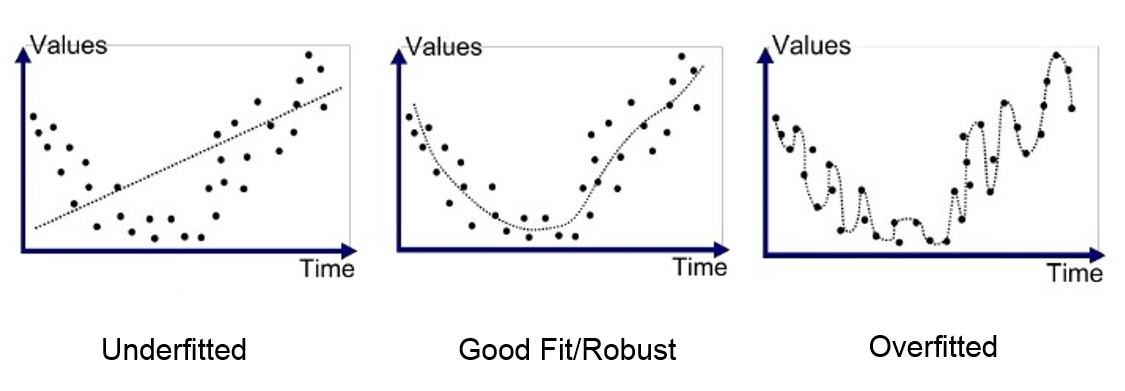
\includegraphics[width=\textwidth]{C:/mimic-iii-project/plots/Useful_plots/overfit.png}
\caption{Ejemplos de sobregeneralización, ajuste adecuado y sobreajuste}
\end{figure}

De esta manera, es necesario encontrar un modelo que no 'memorice' los
datos usados durante su entrenamiento, pero que sea capaz de extraer las
relaciones significativas. No siempre el modelo con mayor precisión
sobre los datos de entreno es el mejor, ya que puede ser un modelo
sobreajustado.

Un modelo sobregeneralizado presenta error alto tanto en los datos de
entreno como en los datos de test, mientras que un modelo sobreajustado
presenta error muy bajo sobre el conjunto de entreno y error alto sobre
el conjunto de test. Será necesario evaluar este factor tras entrenar la red neuronal.

\section{Métricas de evaluación}

El uso correcto de las métricas de evaluación en un modelo
clasificatorio es indispensable para entender el rendimiento de este.

\subsubsection{Precisión de clasificación}

Se trata de la relación entre predicciones correctas y el número total
de predicciones. Es útil cuando las clases a predecir se encuentran
balanceadas, tal como en el caso que nos ocupa. En el caso contrario,
suele inducir a errores de interpretación. Por ejemplo, en una tarea
clasificatoria de imágenes del 0 al 9, si se desea construir un
clasificador que detecte el número 6, basta con que el algoritmo
clasifique cada registro como distinto al 6 para obtener una precisión
del 90\%, ya que solo el 10\% de las imágenes son 6. Esta es una
problemática mayor en tareas de aprendizaje automático y es por ello que
deben emplearse diversas métricas para estudiar un mismo modelo.


\[Precisi\acute{o}n = \frac{\textrm{Predicciones correctas}}{\textrm{Total de predicciones}}\]

\subsubsection{F1 Score}

La precisión, la cual indica el porcentaje de predicciones correctas por
el modelo, y la sensibilidad, que señala que porcentaje de registros
fueron predichos correctamente, se combinan en una misma métrica mediante el 'F1-Score'. Se
calcula a partir de la media harmónica de precisión y sensibilidad, y
por lo tanto, solo devolverá un valor elevado si tanto la sensibilidad
como la precisión son elevadas.

\[F1 =2 * \frac{\textrm{Precisión · Sensibilidad}}{\textrm{Precisión + Sensibilidad}}\]

\subsubsection{Error cuadrático medio}

De forma similar la métrica anterior, mide el promedio de los errores al
cuadrado entre los valores obtenidos y los reales. Se calcula mediante
la siguiente expresión y es conveniente minimizar su valor. Sus siglas
en inglés son MSE (Mean Squared Error).
\begin{equation}
 MSE =\frac{1}{n}\sum_{t=1}^{n}e_t^2
  \label{}
\end{equation}

\subsubsection{AUROC (Area Under Receiver Operating
Characteristic)}
En una curva ROC (Receiver Operating Characteristic) se muestra el ratio
de verdaderos positivos, la sensibilidad, en función del ratio de falsos
positivos, la especificidad. Cada punto de la curva ROC representa la
relación entre sensibilidad y especificad correspondiente a un valor
umbral determinado.

\[Sensibilidad =  \frac{\textrm{Verdaderos positivos + Falsos negativos}}{\textrm{Número de muestras}}\]

\[Especificidad =  \frac{\textrm{Falsos positivos}}{\textrm{Falsos positivos + Verdaderos negativos}}\]

El área bajo esta curva es una medida del grado de ajuste de un
predictor en una tarea de clasificación. Mide la discriminación del
modelo, es decir, la capacidad de clasificar correctamente los valores.
Se considera que un modelo tiene una capacidad de predicción perfecta
cuando este valor es 1, y aleatoria cuando es 0.5.

Es la medida de evaluación más significativa y se emplea a habitualmente para comparar el desempeño de modelos predictivos. 

\section{Parámetros e hiperparámetros}

Los hiperparámetros son las variables que determinan la estructura de la
red neuronal, tal como el número de capas ocultas, y las variables que
determinan como la red se entrena, por ejemplo el ratio de aprendizaje.

Los hiperparámetros se establecen antes de entrenar el modelo y
determinan su rendimiento. Los principales hiperparámetros a seleccionar
son los siguientes:

\begin{itemize}
\item
  Número de capas ocultas y unidades: Se trata de las capas entre la
  capa de entrada y la capa de salida. Un número muy elevado de unidades
  en una misma capa junto con técnicas de regularización permite
  aumentar la precisión del modelo. Sin embargo, un número bajo de
  unidades puede llevar a la sobregeneralización del modelo.
\item
  Dropout: Es una técnica para reducir el sobreajuste en redes
  neuronales. Consiste en desactivar aleatoriamente un porcentaje de
  neuronas en cada capa, con tal de disminuir su peso alternativamente
  en el modelo. De esta forma, la red aumenta su capacidad de
  generalizar los resultados.

\item
  Función de activación: Se emplean para introducir no-linealidades en
  el modelo, lo cual permite al modelo de aprendizaje automático diseñar
  fronteras de predicción no lineales. Se suele emplear generalmente la
  función de rectificación de activación (ReLu). La función sigmoide es
  empleada en la capa de salida en modelos predictivos binarios,
  mientras que la capa 'Softmax' se emplea en modelos predictivos
  multiclase. 

\begin{figure}[H]
\centering
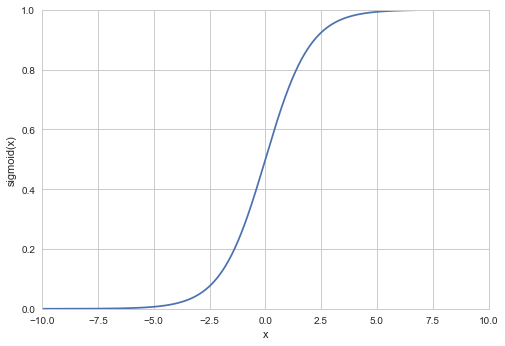
\includegraphics[scale = 0.4]{C:/mimic-iii-project/plots/Useful_plots/sigmoid.png}
\caption{Función de activación sigmoide}
\end{figure}

\item
  Ratio de aprendizaje: Determina la velocidad de actualización de
  parámetros de una red. Un ratio de aprendizaje bajo alentece el
  proceso de aprendizaje, pero converge adecuadamente. Sin embargo, un
  ratio de aprendizaje alto acelera el entreno de la red, pero puede no
  llegar a los parámetros óptimos. Es por esto que se suelen emplear
  ratios de aprendizaje adaptativos, es decir, elevados al inicio del
  entreno de la red y lento una vez se acerca la convergencia. 
\item
  Momento: Permite deducir la dirección del siguiente paso hacia la
  convergencia de la red a partir de los pasos anteriores, evitando así
  oscilaciones en el camino hacia los parámetros óptimos. 
\item
  Epochs: Es la cantidad de veces que el conjunto de datos de
  entrenamiento es proporcionado a la red durante el entreno. 
\item
  Batch Size: Es el número de muestras del conjunto de entreno tras el
  cual se actualizan los parámetros de la red. 
\item
  Algoritmo de optimización: Se trata del algoritmo empleado para
  actualizar los parámetros del modelo, principalmente los pesos y
  varianzas de cada neurona. 
\end{itemize}


\subsection{Ajuste de parámetros e hiperparámetros}

La elección de los parámetros óptimos de una red neuronal es un proceso
esencial en la obtención de un buen modelo predictivo. Existen diversos
enfoques para encontrar estos valores.

\begin{itemize}
\item
  Grid Search: Consiste en probar todas las combinaciones posibles de
  parámetros hasta dar con aquella que minimiza la métrica de evaluación
  empleada. Es un método poco óptimo, únicamente útil en modelos
  sencillos y rápidos de compilar, ya que en el caso contrario requiere
  demasiado tiempo y recursos computacionales. 
\item
  Búsqueda aleatoria: Se trata de probar aleatoriamente combinaciones de
  hiperparámetros hasta dar con alguna que devuelva un resultado
  adecuado. No garantiza encontrar los hiperparámetros óptimos.
\item
  Búsqueda informada: Se buscan los hiperparámetros óptimos evaluando
  tras cada iteraciones el resultado obtenido. Tras cada iteracion, se
  decrece la probabilidad de escoger valores que no corresponden a la
  solución óptima. De esta forma, se escoge un nuevo conjunto de
  parámetros, se observa si se ha aumentado o disminuido la calidad del
  modelo, y acorde a esto, se escoge un nuevo conjunto de parámetros en
  función de los anteriores. De esta manera, se optimiza la búsqueda de
  parámetros, ya que cada paso de cálculo se aproxima cada vez a los
  parámetros óptimos, además de no ser necesario evaluar todas las
  combinaciones de parámetros posibles. 
\end{itemize}

\subsection{Optimización Bayesiana}

Se realiza el ajuste de parámetros mediante la opción de búsqueda
informada, en concreto, emplearemos la optimización Bayesiana.
Es un enfoque basado en modelos probabilísticos para encontrar el mínimo
de una función que devuelve una métrica real. En este caso, la función
es multidimensional, ya que recibe como entrada un espacio de
hiperparámetros. La optimización Bayesiana reduce el número de veces que
debemos entrenar y evaluar la red neuronal, proceso computacionalmente
costoso. Se construye un modelo probabilístico de la función objetivo
que busca la correspondencia entre los valores de entrada, en este caso
los hiperparámetors, y la salida, la métrica de evaluación. De esta
manera, se recalcula la selección de hiperparámetros basándose en la
nueva evidencia encontrada tras cada iteración.

Para la implementación de este método utilizamos la librería Hyperopt.
{[}https://github.com/hyperopt/hyperopt{]}.

Primeramente diseñamos una función que permite entrenar la red neuronal
partir de los parámetros de entrada y devuelve una métrica de
evaluación, el AUROC, definido anteriormente. En este caso, como el
método de optimización Bayesiana busca minimizar la función coste, se
devuelve 1 - AUROC.

Se observa que el modelo recibe como parámetros el número de capas, el número de neuronas por capa, el batch size, el número de epochs y la función de optimización.
Empleamos el modulo roc\_auc\_score de la librería Scikit-Learn para obtener la métrica AUROC, ya que no se encuentra incluida por defecto en Keras. 

Envolvemos está función en una función objetivo, que recibe únicamente los parámetros y devuelve la métrica seleccionada, para ser utilizada por Hyperopt:
\begin{lstlisting}
def f(params):
    return train_neural_network(X_train, Y_train, X_test, Y_test, params);
\end{lstlisting}
\newpage
Posteriormente definimos el espacio de hiperparámetros en el cual buscaremos aquellos óptimos, que maximizen el AUROC del modelo.  En concreto, se prueban los siguientes parámetros.

\begin{itemize}
\item Número de capas: de 2 a 8.
\item Número de neuronas: 8, 16, 32, 64.
\item Funciones de optimización: 'Stochastic Gradient Descent, Adam, RMSProp, Adagrad.
\item Epochs: 10, 25, 35
\item Batch size: 1, 25, 50
\end{itemize}

Se utiliza el algoritmo por defecto de Hyperopt, TPE (Tree-structured Parzen Estimator), el cual explora inteligentemente el espacio de hiperparámetros reduciendo la búsqueda a aquellos óptimos tras cada iteración. 
Tras 50 iteraciones y un tiempo de ejecución de 3.5 horas, obtenemos que los parámetros que maximizan el AUROC son los siguientes:

\begin{itemize}
\item Número de capas: 6
\item Neuronas por capa: 8
\item Batch Size: 50
\item  Epoch: 25
\item Función de optimización: Adam
\end{itemize}

\section{Arquitectura y parámetros escogidos}

Empleando los parámetros obtenidos anteriormente mediante optimización bayesiana, obtenemos la siguiente arquitectura de red, consistente en seis capas totalmente conectadas con 16 neuronas por capa. La capa de entrada es un vector de 101 elementos, tantos como variables de entrada tras su procesado, aunque para representarlo visualmente se muestra como un único nodo. 

\begin{figure}[h]
\centering
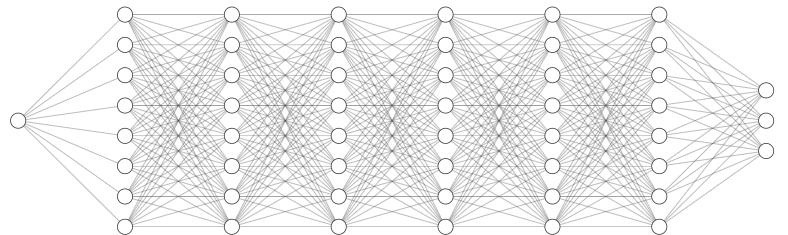
\includegraphics[width = \textwidth]{C:/mimic-iii-project/plots/arquitectura.png}
\caption{Arquitectura de la red neuronal}
\end{figure}
Una vez entrenada y evaluada la red, se juzgará la necesidad de añadir
capas Dropout para regular el sobreajuste, si lo hubiera.
Se utiliza la función activación 'ReLU' , Rectified Linear Unit. Esta
función evita el problema de los gradientes desvanecientes. La red
neuronal calcula los pesos de los parámetros a partir de la diferencia
en la salida del modelo en función de estos. Ciertas funciones de
activación comprimen el resultado en un rango determinado, por ejemplo
{[}-1, 1 {]} en el caso de la tangente hiperbólica. De esta forma, al
entrenar los parámetros de las primeras capas de la red mediante
propagación hacia atrás, la convergencia de los parámetros de estas
capas se hace muy lenta, debido a que los cambios de parámetros producen
efectos negligibles sobre la salida de la red.

La función de activación ReLu evita este problema, ya que no restringe
la salida de la capa a un rango determinado, sinó que permite valores en
el intervalo \{0, $\infty$\}.

También reduce la carga computacional en función a otras funciones, ya
que su cálculo es sencillo e inmediato, sin requerir funciones
trigonométricas o exponenciales. Esto permite entrenar la red más
rápido.
\begin{figure}[H]
\centering
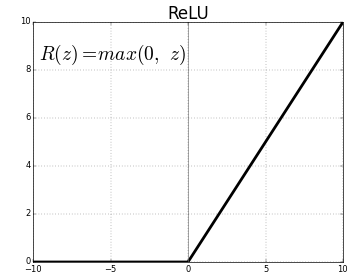
\includegraphics[scale = 0.6]{C:/mimic-iii-project/plots/Useful_plots/relu.png}
\caption{Función de activación ReLu}
\end{figure}
En cuanto al algoritmo de optimización, utilizaremos la función 'Adam',
basado en la adaptación estimada del momento. Fue presentado en 2015 por
investigadores de la Universidad de Toronto. El método computa el ratio
de aprendizaje de la red de forma adaptativa para diferentes parámetros
a partir de estimaciones del primer y segundo momento de los gradientes.
Combina las ventajas de otras extensiones del método clásico, el
algoritmo Stochastic Gradient Descent. Los resultados empíricos muestran
que Adam funciona correctamente en la práctica y se compara
favorablemente con otros métodos estocásticos de optimización.

\begin{figure}[H]
\centering
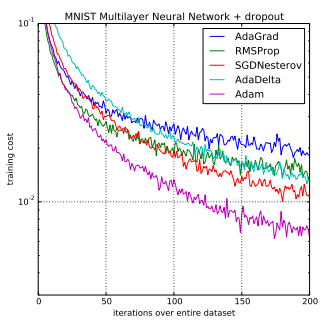
\includegraphics[scale = 0.70]{C:/mimic-iii-project/plots/Useful_plots/optomization_algorithms.png}
\caption{Comparativa de rendimiento entre algoritmos de optimización}
\end{figure}

Por otra parte, haremos 25 pasadas del conjunto de datos durante el
entreno de la red neuronal y actualizaremos los parámetros cada 50
muestras, empleando los valores óptimos de epoch y batch size obtenidos
en el paso anterior.
\newpage
\section{Evaluación del modelo}
Una vez escogidos los parámetros para la red, es conveniente evaluar su
rendimiento a partir de sus métricas de evaluación, además de determinar
si se produce el sobreajuste a los datos de entreno.
\begin{longtable}[]{@{}ll@{}}
\toprule
Métrica & Valor\tabularnewline
\midrule
\endhead
Precisión sobre datos de entreno & 0.656\tabularnewline
Precisión sobre datos de test & 0.632\tabularnewline
Error cuadrático medio & 0.154\tabularnewline
AUROC & 0.812\tabularnewline
\bottomrule
\end{longtable}
Observamos que la red no produce ni sobreajuste ni sobregeneralización,
ya que como es correcto, la precisión sobre los datos de entreno es
ligeramente mayor a la precisión sobre los datos de evaluación.

Calculamos por separado el AUROC para cada una de las tres clases
predichas y representamos sus curvas:

\begin{longtable}[]{@{}lll@{}}
\toprule
Clase & Mortalidad & AUROC\tabularnewline
\midrule
\endhead
0 & \textless{} 1 mes & 0.89\tabularnewline
1 & 1 - 12 meses & 0.72\tabularnewline
2 & \textgreater{} 12 meses & 0.81\tabularnewline
\bottomrule
\end{longtable}
\begin{figure}[H]
\centering
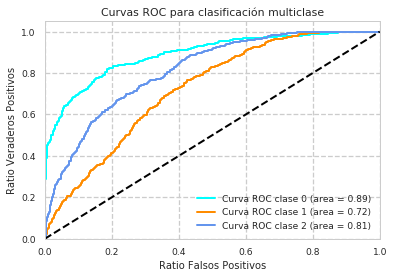
\includegraphics[scale = 0.70]{C:/mimic-iii-project/plots/Evaluation/3Curvas_SPA.png}
\caption{Curvas AUROC}
\end{figure}

El AUROC combinado de las tres clases obtenido indica que se trata de un
buen modelo, con buena capacidad diagnóstica, especialmente en la clase
con mayor valor médico, la de los pacientes que fallecen antes de un mes
de su alta hospitalaria. Obtenemos una capacidad predictoria también
buena para la clase superior a un año, aunque moderada para el grupo de
entre 1 y 12 meses.

En cuanto a la matriz de confusión normalizada del modelo, obtenemos el
siguiente resultado:

\begin{figure}[H]
\centering
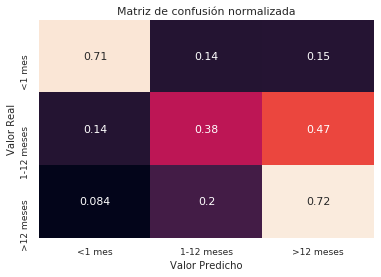
\includegraphics[scale = 0.70]{C:/mimic-iii-project/plots/Evaluation/matriz_confusion_normalizada_seaborn.png}
\caption{Matriz de confusión}
\end{figure}

De nuevo, se observa que el modelo posee dificultades para discernir
pacientes en el intervalo de 1 a 12 meses, aunque no lo hace para las
otras dos clases.
El reporte de métricas de evaluación para las tres clases es el
siguiente.

\begin{longtable}[]{@{}llll@{}}
\toprule
Clase & Precisión & Recall & F1 Score\tabularnewline
\midrule
\endhead
\textless{}1 mes & 0.79 & 0.71 & 0.75\tabularnewline
1 - 12 meses & 0.47 & 0.38 & 0.42\tabularnewline
\textgreater{}12 meses & 0.57 & 0.72 & 0.64\tabularnewline
\bottomrule
\end{longtable}

\section{Ejemplo de uso}
Para utilizar el modelo para hacer predicciones se debe realizar el
siguiente procedimiento.
Primeramente hay que proporcionar información categórica relacionada con
el paciente y su estancia a través de un objeto:

\begin{verbatim}
patient_categorical_features = {'gender': 'M',
                                'marital_status':'SINGLE',
                                'religion':'CHRISTIAN',
                                'ethnicity':'WHITE',
                                'service':'CSURG',
                                'icd9_group':'diseases of the circulatory system',
                                'SURGERY_FLAG':'NARROW'
                                };
\end{verbatim}

Y en otros dos objetos, los resultados de los test de laboratorios y señales fisiológicos. Cada variable se debe introducir como un arreglo de elementos, del cual posteriormente se calcula el promedio y la desviación estándar. Las unidades de cada una se hayan también descritas en el apartado 'Variables predictorias'.

\begin{verbatim}
patient_lab_tests = {'blood_urea_nitrogen': [23, 24, 24],
                     'platelet_count':[230, 240],
                     'hematocrit':[33, 35],
                     'potassium': [3.9,3.8,4.4],
                     'sodium':[140, 139],
                     'creatinine':[1.3,1.2,1.3],
                     'bicarbonate':[25,26],
                     'white_blood_cells':[8.5,9,13],
                     'blood_glucose':[130, 135,140],
                     'albumin':[3.5, 3.4] };
                    

patient_physio_measures = {'heart_rate':[100,108,105,99],
                           'resp_rate':[22,25,23],
                           'sys_press':[120, 121, 115],
                           'días_press':[70,80,85],
                           'temp':[98, 98.2, 97.8],
                           'spo2':[97,97.8,98] };
              
\end{verbatim}
Posteriormente emplearemos la función preprocess\_prediction\_data, a la cual suministraremos las carácterísticas del paciente en forma de objeto, las variables numéricas con los valores faltantes previamente imputados y las variables categóricas. De esta forma, en caso de que hayan valores faltantes, por ejemplo si no se ha tomado la temperatura del paciente, podremos imputarlos mediante el método MICE anteriormente definido.

\begin{verbatim}
prediction_data = NeuralNetworkService().preprocess_prediction_data(
    patient_features,
    imputed_numerical_features,
    categorical_features
	);
\end{verbatim}
Esta función nos devuelve las variables predictorias del paciente tratadas para ser introducidas en el modelo. En concreto, se han normalizado las variables numéricas, imputado valores faltantes y categorizado las variables numéricas. Empleando estos valores, realizamos la predicción seguidamente:

\begin{verbatim}
prediction = keras_model.predict(prediction_data);
\end{verbatim}

Para este paciente, el resultado de la predicción nos devuelve las siguientes probabilidades por clase: 

\begin{longtable}[]{@{}lll@{}}
\toprule
\textless{} 1 mes & 1 - 12 meses & \textgreater{} 12
meses\tabularnewline
\midrule
\endhead
0.54086 & 0.27766 & 0.18148\tabularnewline
\bottomrule
\end{longtable}
Viendo este resultado, el personal médico debería valorar la decisión de dar el alta al paciente, debido a su alto riesgo de fallecer antes de un més tras su salida del hospital.
\newpage
\section{Comparativa de rendimiento}

En esta sección, se compara la capacidad predictiva del modelo aquí desarrollado con otros estudios del ámbito de la predicción de destinos médicos.

\paragraph{Mortality prediction in intensive care units with the Super ICU Learner Algorithm (SICULA): a population-based study.} Este estudio emplea diversas técnicas combinadas de aprendizaje automático para predecir la mortalidad hospitalaria de pacientes críticos. Emplea la versión II de la base de datos MIMIC, anterior a la utilizada aquí. Emplea las 17 variables utilizadas por los indicadores de severidad SAPS II y SOFA, a los cuales supera ampliamente en capacidad predictiva. En concreto, llega a conseguir un AUROC del 0.94 para la predicción de mortalidad hospitalaria. 
De esta forma, presenta un poder predictivo superior a la red neuronal diseñada en este trabajo, aunque tratándose de predicción de mortalidad hospitalaria en lugar de extrahospitalaria.
\begin{itemize}
\item{Pirracchio R, Petersen ML, Carone M, Rigon MR, Chevret S, van der LAAN MJ. Mortality prediction in the ICU: can we do better? Results from the Super ICU Learner Algorithm (SICULA) project, a population-based study. The Lancet Respiratory medicine. 2015;3(1):42-52. doi:10.1016/S2213-2600(14)70239-5.}
\end{itemize}
\paragraph{Mortality prediction with self normalizing neural networks in intensive care unit patients} Este estudio, realizado por investigadores de la Universidad de Waterloo, Canadá, en Abril de 2018,  se centra en la predicción de la mortalidad hospitalaria y la mortalidad a 30 dias, también estudiada en este trabajo. Utiliza la base de datos MIMIC II y evalúa el modelo sobre 17.000 pacientes, obteniendo un AUROC del 0.84 para la mortalidad a 30 dias y del 0.86 para la mortalidad hospitalaria. Para ello, emplea una red neuronal autonormalizante. Estas redes se caracterizan por mantener la normalización de las activaciones durante su propagación a través de las capas de la red, para lo cual se emplea la función de activación 'SELU'  (Scaled Exponential Linear Units).
El AUROC conseguido mediante esta técnica es inferior al obtenido en este trabajo para la misma tarea de predicción de mortalidad a 30 días. (0.84 vs. 0.89)

\begin{itemize}
\item M. A. H. Zahid and J. Lee, "Mortality prediction with self normalizing neural networks in intensive care unit patients," 2018 IEEE EMBS International Conference on Biomedical \& Health Informatics (BHI), Las Vegas, NV, 2018, pp. 226-229.
doi: 10.1109/BHI.2018.8333410
\end{itemize}

\paragraph{A machine learning approach to predicting short-term mortality risk for patients starting chemotherapy.}

En este documento se emplean árboles de decisión de gradiente potenciado (Gradiend Boosted Decision Trees) sobre un conjunto de datos consistente en alrededor de 27.000 pacientes que recibieron quimioterápia entre 2004 y 2014 en el centro 'Dana-Farber/Brighan and Woman's Cancer Center', en Boston, Massachusetts. Se diseña un modelo capaz de predecir la mortalidad a 30 días tras el inicio de un tratamiento de quimioterápia utilizando información demográfica, medicación recibida, comorbilidades, grupos de diagnóstico ICD-9, señales vitales, resultados de laboratorio y datos extraídos de anotaciones médicas, obteniendo un AUROC del 0.94, superior al obtenido en este trabajo para el mismo íntervalo de tiempo.

\begin{itemize}
\item A machine learning approach to predicting short-term mortality risk for patients starting chemotherapy.
Ravi Bharat Parikh, Aymen Elfiky, Maximilian J. Pany, and Ziad Obermeyer
Journal of Clinical Oncology 2017 35:15 suppl, 6538-6538 
\end{itemize}

\chapter*{Conclusiones}

Se ha desarrollado satisfactoriamente un modelo predictivo de la
mortalidad extrahospitalaria con una buena capacidad diagnóstica.
Este proyecto ha comportado la exploración de una gran base de datos con
muchos tipos de valores diferentes: numéricos, categóricos, fechas,
campos de texto, etc, y el tratamiento de ellos para ser procesados por
la red neuronal.

Las variables necesarias para realizar predicciones con este modelo son
fáciles de obtener y se recopilan de forma rutinaria, lo cual permitiría
un uso extendido del algoritmo en la práctica médica, aunque siempre
considerando que comete ciertas inexactitudes. Podría llegar a emplearse
como segunda opinión médica, para confirmar o cancelar el alta de
pacientes en unidad de cuidados intensivos.

La mayor carga de trabajo ha recaído sobre la selección, extracción y
preprocesado de las variables empleadas por el modelo. Este proceso a
llevado al descarte de ciertas variables, por ejemplo la presión venosa
central, por disponerse de pocas muestras.

Por otra parte, gracias a la optimización bayesiana de hiperparámetros
ha sido relativamente sencillo, aunque lento, encontrar la configuración
de red que asegura un resultado óptimo.

Como mejoras, se podrían extraer nuevas variables ignoradas en este
estudio. Por ejemplo, en la base de datos se almacenan las notas médicas
como campo libre de texto para cada paciente, las cuales incluyen
anotaciones realizadas por el personal médico acerca del historial de
los pacientes o situaciones médicas particulares. La extracción de estas
características supondría un amplio trabajo de minería de textos que cae
fuera del alcance de este proyecto, pero podría mejorar ampliamente la capacidad predictoria del modelo aquí diseñado.

Así mismo, sería posible desarrollar una pequeña interfaz o página web
que permita realizar predicciones empleando el modelo diseñado. Esta
interfaz permitiría al personal médico la introducción de las variables
necesarias y devolvería la probabilidad de mortalidad del paciente.

\chapter{Análisis económico}
El mayor coste económico de este proyecto recae en el sueldo del
ingeniero que ha desarrollado la red neuronal que llevará a cabo la
predicción de mortalidad. De esta manera, la mayor parte del coste
económico irá destinada a pagar sus horas de trabajo, y otra pequeña
parte irá a parar el coste indirecto del proyecto, consistente
principalmente en el equipo informático que utiliza.

\section{Costes directos}
Son aquellos costes que pueden identificarse directamente con un objeto
de costes, tal como materiales o mano de obra destinada al proyecto.

En este caso, el coste directo es completamente el sueldo del personal,
al cual consideramos un trabajador autónomo que factura por horas.

Consideramos que el proyecto lo ha llevado a cabo un único desarrollador, con una facturación de 30\euro/h y una dedicación de 320h,
dando de esta manera un coste directo total de 9600\euro.
\section{Costes indirectos}
El coste indirecto del proyecto corresponde al equipo informático
empleado.

No existen costes asociados al software, ya que Python es un lenguaje de
programación gratuito de código abierto y el sistema operativo del
equipo es Elementary OS loki 0.4.1, distribución de Linux basada en
Ubuntu y también gratuita.

En cuando al hardware, se emplea un ordenador portátil del siguiente
modelo:

\begin{itemize}
\item
  Toshiba Satellite Pro A50-D-1FZ Intel Core i7-7500U/8GB/256GB
  SSD/15.6" 
\end{itemize}

Su coste es de 695\euro. Considerando un periodo de amortización de tres
años y un periodo de uso de cuatro meses, el coste indirecto de hardware
es de 77.22 \euro.

De esta manera, el coste total del proyecto computado como la suma de
costes directos e indirectos es de alrededor de 9700 \euro.

\chapter{Análisis del impacto ambiental}
El impacto ambiental del desarrollo del estudio es negligible,
consistente únicamente en la electricidad consumida por el ordenador.

Por otra parte, considerando que el modelo predictivo aquí desarrollado
llega a ser implementado en la práctica médica y permite prevenir el
fallecimiento prematuro del 5\% de pacientes, podemos estimar el impacto
ambiental del proyecto a partir de la contaminación que generan.

Según datos del INE en 2014 cada español genera 459 kilos de residuos y
5.08 toneladas métricas de dióxido de carbono anualmente. Así mismo,
consume un promedio de 132 litros de agua diarios, lo cual supone
alrededor de 48 toneladas de agua al año.

Cada año son ingresados 1200 pacientes en la unidad de cuidados
intensivos del Hospital Vall d'Hebron de Barcelona.

De esta forma, el impacto ambiental anual del proyecto, en caso de
implementarse el modelo predictivo en tal hospital y alargando la vida
de 60 de los pacientes, sería el siguiente:

\begin{itemize}
\item
  27.5 toneladas de residuos
\item
  305 toneladas de CO2
\item
  2900 toneladas de agua
\end{itemize}

\chapter{Bibliografía}
\begin{itemize}

\item
  Pirracchio R, Petersen ML, Carone M, Rigon MR, Chevret S, van der LAAN
  MJ. Mortality prediction in the ICU: can we do better? Results from
  the Super ICU Learner Algorithm (SICULA) project, a population-based
  study. \emph{The Lancet Respiratory medicine}. 2015;3(1):42-52.
  doi:10.1016/S2213-2600(14)70239-5.

\item
  Aya Awad, Mohamed Bader-El-Den, James McNicholas, Jim Briggs. Early
  hospital mortality prediction of intensive care unit patients using an
  ensemble learning approach. .Int J Med Inform. 2017 Dec; 108:
  185--195. Published online 2017 Oct 5. doi:
  10.1016/j.ijmedinf.2017.10.002

\item
  MIMIC Code Repository. Cambridge: Laboratory for Computational
  Physiology, Massachusetts Institute of Technology; 2018 {[}updated
  March 15, 2018{]}. Disponible en: http://
  github.com/MIT-LCP/mimic-code. Consultado el 15 mayo de 2018.

\item
  Johnson AE, Pollard TJ, Shen L, et al. MIMIC-III, a freely accessible
  critical care database. Sci Data. 2016;3:160035.
  {[}http://dx.doi.org/10.13026/C2XW26{]} (2016)

\item
  Azur MJ, Stuart EA, Frangakis C, Leaf PJ. Multiple Imputation by
  Chained Equations: What is it and how does it work?
  \emph{International journal of methods in psychiatric research}.
  2011;20(1):40-49. doi:10.1002/mpr.329.

\item
  Pastur-Romay LA, Cedrón F, Pazos A, Porto-Pazos AB. Deep Artificial
  Neural Networks and Neuromorphic Chips for Big Data Analysis:
  Pharmaceutical and Bioinformatics Applications. González-Díaz H,
  Todeschini R, Pazos Sierra A, Arrasate Gil S, eds. \emph{International
  Journal of Molecular Sciences}. 2016;17(8):1313.
  doi:10.3390/ijms17081313.

\item
  Moreno RP, Metnitz PGH, Almeida E, et al. SAPS 3-\/-From evaluation of
  the patient to evaluation of the intensive care unit. Part 2:
  Development of a prognostic model for hospital mortality at ICU
  admission. Intensive Care Med. 2005;31:1345--55.   {[}https://www.ncbi.nlm.nih.gov/pubmed/16132892{]}  
\item
  Awad, Aya et al. ``Early hospital mortality prediction of intensive
  care unit patients using an ensemble learning approach.''
  \emph{International journal of medical informatics} 108 (2017):
  185-195 .

\item
  Knaus WA, Wagner DP, Draper EA, et al. The APACHE III prognostic
  system. Risk prediction of hospital mortality for critically ill
  hospitalized adults. Chest. 1991;100:1619-- 36.
{[}https://www.ncbi.nlm.nih.gov/pubmed/1959406{]}  

\item
  Cook NR. Use and misuse of the receiver operating characteristic curve
  in risk prediction. Circulation. 2007;115:928--35.
{[}https://www.ncbi.nlm.nih.gov/pubmed/17309939{]}  
\item
  Knaus WA, Harrell FE, Fisher CJ, et al. The clinical evaluation of new
  drugs for sepsis: a prospective analysis based on survival analysis.
  JAMA 1993; 270: 1233-41.
\item
  W.G. Baxt. Application of artificial neural networks to clinical
  medicine. Lancet, 346 (2007), pp. 1135-1138
\item
  P.O. Lang, D. Zekry, J.P. Michel, M. Drame, J.L. Novella, D. Jolly,
  *et al. Early markers of prolonged hospital stay in demented
  inpatients: a multicentre and prospective study. J Nutr Health Aging,
  14 (2010), pp. 141-147-
\item
  S.W. Meldon, L.C. Mion, R.M. Palmer, B.L. Drew, J.T. Connor, L.J.
  Lewicki, *et al. A brief risk-stratification tool to predict repeat
  emergency department visits and hospitalizations in older patients
  discharged from the emergency department. Acad Emerg Med, 10 (2003),
  pp. 224-232
\item
  Lokhandwala S, McCague N, Chahin A, Escobar B, Feng M, Ghassemi MM,
  Stone DJ, Celi LA.  {One-year mortality after recovery from critical illness: A retrospective cohort study}.
  PLoS ONE, 13(5):e0197226, May 2018. 

\end{itemize}

\chapter*{Anexos}
\addcontentsline{toc}{chapter}{Anexos}

\section{Código empleado}

A continuación se muestran los fragmentos de código más relevantes empleados en este estudio. El código completo se encuentra en el repositorio de Github del proyecto:  [https://github.com/DanielSola/mimic-iii-project]

\paragraph{Ajuste de hiperparámetros y entreno del modelo}

Determinación de los parámetros óptimos mediante la librería Hyperopt y entreno del modelo. 

\begin{verbatim}
from services.plotting_service import *
from services.neural_network_service import *
from services.preprocessing_service import *
from features.get_features import *
from keras.optimizers import SGD, Adam, RMSprop, Adagrad
from hyperopt import hp, Trials, fmin, tpe

#Query and prepreocess data
nn_data =  NeuralNetworkService().get_nn_data();
categorical_features = Features().get_categorical_features();
numerical_features = Features().get_numerical_features();
imputed_numerical_features = impute_missing_values(numerical_features);

#Split into training and test set
X_train = nn_data['mortality_data']['X_train'];
X_test = nn_data['mortality_data']['X_test'];
Y_train = nn_data['mortality_data']['Y_train'];
Y_test = nn_data['mortality_data']['Y_test'];

#Hyperparameter tuning by Bayesian optimization
def f(params):
    return train_neural_newtork(X_train, Y_train, X_test, Y_test, params);

params_space = {'n_layers': hp.choice('n_layers', range(2,8)),
                    'n_neurons': hp.choice('n_neurons', [8, 16, 32, 64]),
                    'optimizer': hp.choice('optimizer', ['SGD', 'Adam', 'RMSprop', 'Adagrad']),
                    'epochs': hp.choice('epochs', [10, 25, 35]),
                    'batch_size': hp.choice('batch_size', [1, 25, 50])
                };

trials_mse = Trials()

best = fmin(fn=f, space=params_space, algo=tpe.suggest, max_evals=50, trials=trials_mse);

# Training neural network with optimal parameters
params = {'n_layers':6,
          'n_neurons':16,
          'optimizer': 'Adam',
          'epochs':50,
          'batch_size':50
          };
          
keras_model = NeuralNetworkService().train_neural_network(X_train, Y_train, X_test, Y_test, params);

\end{verbatim}

\paragraph{Realización de predicciones}

Empleamos el modelo previamente entrenado y preprocesamos los datos del paciente con el fin de utilizar el modelo para predecir su mortalidad extrahospitalaria.

\begin{verbatim}
#Define patient features
patient_categorical_features = {'gender': 'M',
                                 'marital_status':'SINGLE',
                                 'religion':'CHRISTIAN',
                                 'ethnicity':'WHITE',
                                 'service':'CSURG',
                                 'icd9_group':'diseases of the circulatory system',
                                 'SURGERY_FLAG':'NARROW'
                                };
                                
patient_numerical_features = {'age':80,
                              'total_icu_time':10,
                              'total_los_days':12,
                              'admissions_count':3,
                              'procedure_count':4,
                              'oasis_avg':40,
                              'sofa_avg':7,
                              'saps_avg':20,
                              'gcs':9,
                              'total_mech_vent_time':130
                              };

patient_lab_tests = {'blood_urea_nitrogen': [23, 24, 24],
                     'platelet_count':[230, 240],
                     'hematocrit':[33, 35],
                     'potassium': [3.9,3.8,4.4],
                     'sodium':[140, 139],
                     'creatinine':[1.3,1.2,1.3],
                     'bicarbonate':[25,26],
                     'white_blood_cells':[8.5,9,13],
                     'blood_glucose':[130, 135,140],
                     'albumin':[3.5, 3.4]
                     };

patient_physio_measures = {'heart_rate':[100,108,105,99],
                           'resp_rate':[22,25,23],
                           'sys_press':[120, 121, 115],
                           'dias_press':[70,80,85],
                           'temp':[98, 98.2, 97.8],
                           'spo2':[97,97.8,98]
                           };

patient_features = {
        'patient_categorical_features':patient_categorical_features,
        'patient_numerical_features':patient_numerical_features,
        'patient_lab_tests':patient_lab_tests,
        'patient_physio_measures':patient_physio_measures
        };


# Preprocess prediction data and predict
prediction_data = NeuralNetworkService().preprocess_prediction_data(patient_features, imputed_numerical_features, categorical_features);
prediction = keras_model.predict(prediction_data);

\end{verbatim}

\paragraph{Definición de la red neuronal}
Código empleado para entrenar la red neuronal utilizando la librería Keras. 
\begin{verbatim}
    def train_neural_network(self, X_train, Y_train, X_test, Y_test, params):

        n_layers = params['n_layers'];
        n_neurons = params['n_neurons'];
        batch_size = params['batch_size'];
        epochs = params['epochs'];
        optimizer = params['optimizer'];

        #Model definition
        model = Sequential();
        for i in range(n_layers):
            model.add(Dense(n_neurons, activation='relu', input_shape=(101,)))
        model.add(Dense(3, activation='softmax'));
        model.compile(loss='binary_crossentropy',
                  optimizer=optimizer,
                  metrics=['accuracy', 'mse'])
        model.fit(X_train, Y_train,epochs=epochs, batch_size=batch_size, verbose=1);

        #Evaluating model
        Y_pred = model.predict(X_test);
        Y_train_pred = pd.get_dummies(model.predict(X_train).argmax(axis = 1));
        Y_test_pred = pd.get_dummies(Y_pred.argmax(axis = 1));

        #Evaluation metrics logs
        train_accuracy = accuracy_score(Y_train, Y_train_pred);
        test_accuracy = accuracy_score(Y_test, Y_test_pred);
        f1_score_model = f1_score(Y_test_pred, Y_test, average = 'samples');
        loss, accuracy, mse = model.evaluate(X_test, Y_test,verbose=0)
        roc_auroc = roc_auc_score(Y_test, Y_pred);
        print('TRAIN ACCURACY:',train_accuracy,
                'TEST ACCURACY:',test_accuracy,
                'F1 SCORE:', f1_score_model,
                'MSE:',mse,
                'AUROC:', roc_auroc);
        
        return model;
\end{verbatim}


\paragraph{Normalización de variables numéricas}

Ajuste de variables numéricas a $\sigma$ = 1 y $\mu$ = 0 mediante el método scale del módulo preprocessing de 'Scikit-Learn'

\begin{verbatim}
def scale_numerical_features(imputed_numerical_features):
    scaled_numerical_features = pd.DataFrame(preprocessing.scale(imputed_numerical_features));
    scaled_numerical_features.columns = imputed_numerical_features.columns;
    scaled_numerical_features.index = imputed_numerical_features.index;
    
    return scaled_numerical_features;
\end{verbatim}
\newpage
\paragraph{Extracción del servicio médico más relevante}

Función de preprocesado que se aplica sobre un DataFrame de Pandas proveniente de la consulta a base de datos de los servicios médicos por los que pasa un paciente durante su estancia hospitalaria. Devuelve el de mayor releváncia según lo definido anteriormente. 

\begin{verbatim}
def get_relevant_admission_service(hadm_id, services_df):
    
    admission_services = list(services_df.loc[services_df['hadm_id'] == hadm_id].curr_service)
    ##Cirugia especial
    special_surgery_service = list(filter(lambda x: 'SURG' in x and x != "SURG", admission_services)) 
    ##Cirugia general
    general_surgery_service = list(filter(lambda x:  x == 'SURG', admission_services)) 
    ##No medicina general
    specialised_service = list(filter(lambda x:  x != 'MED' and not 'SURG' in x, admission_services)) 
    ##Medicina general
    general_medicine_service = list(filter(lambda x:  x == 'MED', admission_services)) 
    
    if special_surgery_service:
        return (hadm_id, special_surgery_service[0]);
    if general_surgery_service:
        return (hadm_id, general_surgery_service[0]);
    if specialised_service:
        return (hadm_id, specialised_service[0]);
    if general_medicine_service:
        return (hadm_id, general_medicine_service[0]);
\end{verbatim}

\paragraph{Imputación de valores faltantes}

Uso del método MICE de la biblioteca fancyimpute para imputar los valores faltantes.

\begin{verbatim}
def impute_missing_values(numerical_features):
    imputed_numerical_features = pd.DataFrame(MICE().complete(numerical_features));
    imputed_numerical_features.columns = numerical_features.columns;
    imputed_numerical_features.set_index(numerical_features.index, inplace = True);
\end{verbatim}

\paragraph{Eliminación de outliers}

Función que recibe un DataFrame de Pandas y elimina los outliers comprendidos entre 'low\_quantile' y 'high\_quantile' de la columna especificada por 'column\_index'.

\begin{verbatim}
def remove_outliers(data, column_index, low_quantile, high_quantile):
    
    low_quantile_value = float(data.iloc[:, column_index].quantile(low_quantile));
    high_quantile_value = float(data.iloc[:, column_index].quantile(high_quantile));

    data.iloc[:,column_index] = data.iloc[:,column_index].apply(
            lambda x: x if (x <= high_quantile_value and x >= low_quantile_value)  else np.NaN);
    
    return data;
\end{verbatim}
\newpage
\paragraph{Consultas a base de datos}

A continuación se muestran las consultas empleadas para extraer la información de la base de datos, en sintaxis de PostgreSQL.

\begin{verbatim}
AGE_QUERY = """SELECT hadm_id, EXTRACT(epoch FROM (admittime - dob))/(3600*24*365)
               AS age
               FROM admissions a
               INNER JOIN patients p
               ON a.subject_id = p.subject_id"""
               
GENDER_QUERY = """SELECT hadm_id, gender
                  FROM admissions a
                  INNER JOIN patients p
                  ON a.subject_id = p.subject_id"""
               
               
MARITAL_STATUS_QUERY = """SELECT hadm_id, marital_status 
                          FROM admissions a
                          INNER JOIN patients p
                          ON a.subject_id = p.subject_id"""
                          
RELIGION_QUERY = """SELECT hadm_id, religion 
                    FROM admissions a
                    INNER JOIN patients p
                    ON a.subject_id = p.subject_id"""       

ETHNICITY_QUERY = """SELECT hadm_id, ethnicity 
                    FROM admissions a
                    INNER JOIN patients p
                    ON a.subject_id = p.subject_id"""             

                         
                
SERVICE_QUERY = """SELECT hadm_id, curr_service
                    FROM services
                    ORDER BY hadm_id ASC"""
                    
DIAG_ICD9_CODES_QUERY = """SELECT hadm_id, diagnoses_icd.icd9_code
                            FROM diagnoses_icd 
                            WHERE seq_num = 1"""
                            
PROC_ICD9_CODES_QUERY = """ SELECT hadm_id, procedures_icd.icd9_code
                            FROM procedures_icd 
                            INNER JOIN d_icd_procedures
                            ON procedures_icd.icd9_code = d_icd_procedures.icd9_code
                            WHERE hadm_id is not null
                            AND seq_num = 1"""
                            
ICU_LOS_QUERY = """SELECT hadm_id, sum(los) AS total_icu_time 
                   FROM icustays
                   GROUP BY hadm_id
                   ORDER BY hadm_id"""
                   
TOTAL_LOS_QUERY = """SELECT hadm_id, 
                     EXTRACT(epoch FROM(dischtime - admittime))/(3600*24) AS total_los_days
                     FROM admissions"""
                
PREVIOUS_ADMISSIONS_QUERY = """SELECT hadm_id, subject_id, admittime
                               FROM admissions
                               ORDER BY admittime ASC"""
                               
PROCEDURE_COUNT_QUERY = """SELECT hadm_id, count(*) AS procedure_count
                           FROM procedures_icd
                           GROUP BY hadm_id"""
                            
MECHANICAL_VENTILATION_TIME_QUERY = """SELECT hadm_id, SUM(duration_hours) AS total_mech_vent_time
                                       FROM ventdurations v
                                       INNER JOIN icustays i
                                       ON v.icustay_id = i.icustay_id
                                       GROUP BY hadm_id"""
                                        
SEVERITY_SCORES_QUERY = """SELECT o.hadm_id, 
                           AVG(o.oasis) AS oasis_avg, 
                           AVG(so.sofa) AS sofa_avg, 
                           AVG(sa.saps) as saps_avg
                           FROM oasis o
                           INNER JOIN sofa so
                           ON o.hadm_id = so.hadm_id
                           INNER JOIN saps sa
                           ON sa.hadm_id = so.hadm_id
                           GROUP BY o.hadm_id"""
                           
GLASGOW_COMA_SCALE_QUERY = """SELECT hadm_id, AVG(gcs) AS GCS
                              FROM pivoted_gcs gcs
                              INNER JOIN icustays i
                              ON gcs.icustay_id = i.icustay_id
                              GROUP by hadm_id"""

MORTALITY_QUERY = """SELECT hadm_id,
                     CASE
                     WHEN 
                              EXTRACT(epoch FROM (dod-dischtime))/(3600*24*30) >= 12
                     THEN '12+ months'			
                     WHEN 
                        	      EXTRACT(epoch FROM (dod-dischtime))/(3600*24*30) < 12 AND
                               EXTRACT(epoch FROM (dod-dischtime))/(3600*24*30) >= 1

                     THEN '1-12 months'
                     WHEN
                               EXTRACT(epoch FROM (dod-dischtime))/(3600*24*30) < 1 AND
                               EXTRACT(epoch FROM (dod-dischtime))/(3600*24*30) > -0.5
                     THEN '0-1 months'	
									
                     END
                     AS mortality
                     FROM admissions a
                     INNER JOIN patients p
                     ON a.subject_id = p.subject_id
                     WHERE p.expire_flag = 1
                 """
                                 
                                
ADMISSION_DATA_QUERY = """SELECT hadm_id, p.subject_id, admittime, dischtime
                          FROM admissions a 
                          INNER JOIN patients p
                          ON a.subject_id = p.subject_id
                          WHERE EXTRACT(epoch FROM (a.admittime - p.dob)) / (365 * 24 * 3600) BETWEEN 18 AND 80
                          ORDER BY subject_id ASC"""
                            
MORTALITY_TIME_QUERY = """SELECT hadm_id, EXTRACT(epoch FROM (dod-dischtime))/(3600*24) AS expire_days 
                          FROM admissions a
                          INNER JOIN patients p
                          ON a.subject_id = p.subject_id
                          WHERE EXTRACT(epoch FROM (dod-dischtime))/(3600*24) > 0.5
                          AND p.expire_flag = 1"""

HOSPITAL_EXPIRE_FLAG_QUERY = """SELECT hadm_id, hospital_expire_flag 
                                FROM admissions"""
\end{verbatim}

\paragraph{Agrupación de códigos ICD-9 de diagnóstico} Función que devuelve el grupo de código de diagnóstico ICD9 principal a partir del código detallado de diagnóstico. 

\begin{verbatim}
def group_diag_icd9_code(icd9_code):
    if not 'V' in icd9_code and not 'E' in icd9_code:
        truncated_code = int((icd9_code)[0:3]);
        if truncated_code > 0 and truncated_code <= 139:
            return 'infectious and parasitic diseases';
        if truncated_code > 139 and truncated_code <= 239:
            return 'neoplasms';
        if truncated_code > 239 and truncated_code <= 279:
            return 'endocrine, nutritional and metabolic diseases, and immunity disorders';
        if truncated_code > 279 and truncated_code <= 289:
            return 'diseases of the blood and blood-forming organs';
        if truncated_code > 289 and truncated_code <= 320:
            return 'mental disorders';
        if truncated_code > 320 and truncated_code <= 389:
            return 'diseases of the nervous system and sense organs';
        if truncated_code > 389 and truncated_code <= 459:
            return 'diseases of the circulatory system';
        if truncated_code > 459 and truncated_code <= 519:
            return 'diseases of the respiratory system';
        if truncated_code > 519 and truncated_code <= 579:
            return 'diseases of the digestive system';
        if truncated_code > 579 and truncated_code <= 629:
            return 'diseases of the genitourinary system';
        if truncated_code > 629 and truncated_code <= 679:
            return 'complications of pregnancy, childbirth, and the puerperium';
        if truncated_code > 679 and truncated_code <= 709:
            return 'diseases of the skin and subcutaneous tissue';
        if truncated_code > 709 and truncated_code <= 739:
            return 'diseases of the musculoskeletal system and connective tissue';
        if truncated_code > 739 and truncated_code <= 759:
            return 'congenital anomalies';
        if truncated_code > 759 and truncated_code <= 779:
            return 'certain conditions originating in the perinatal period';        
        if truncated_code > 779 and truncated_code <= 799:
            return 'symptoms, signs, and ill-defined conditions';       
        if truncated_code > 799 and truncated_code <= 999:
            return 'injury and poisoning';                         
    if 'E' in icd9_code: 
        return 'external causes of injury';
    if 'V' in icd9_code: 
        return 'supplementary classification of factors influencing health status';    
\end{verbatim}

\end{document}

